%% Copyright 2007-2020 Elsevier Ltd
%% 
%% This file is part of the 'Elsarticle Bundle'.
%% ---------------------------------------------
%% 
%% It may be distributed under the conditions of the LaTeX Project Public
%% License, either version 1.2 of this license or (at your option) any
%% later version.  The latest version of this license is in
%%    http://www.latex-project.org/lppl.txt
%% and version 1.2 or later is part of all distributions of LaTeX
%% version 1999/12/01 or later.
%% 
%% The list of all files belonging to the 'Elsarticle Bundle' is
%% given in the file `manifest.txt'.
%% 

%% Template article for Elsevier's document class `elsarticle'
%% with numbered style bibliographic references
%% SP 2008/03/01
%%
%% 
%%
%% $Id: elsarticle-template-num.tex 190 2020-11-23 11:12:32Z rishi $
%%
%%
\documentclass[final,a4paper]{elsarticle}
\usepackage[centering,top=1in,bottom=1in,left=1in,right=1in]{geometry}
\usepackage[dvipsnames]{xcolor}
\geometry{letterpaper}
% \documentclass[preprint,12pt]{elsarticle}

%% Use the option review to obtain double line spacing
%% \documentclass[authoryear,preprint,review,12pt]{elsarticle}

%% Use the options 1p,twocolumn; 3p; 3p,twocolumn; 5p; or 5p,twocolumn
%% for a journal layout:
%% \documentclass[final,1p,times]{elsarticle}
%% \documentclass[final,1p,times,twocolumn]{elsarticle}
%% \documentclass[final,3p,times]{elsarticle}
%% \documentclass[final,3p,times,twocolumn]{elsarticle}
%% \documentclass[final,5p,times]{elsarticle}
%% \documentclass[final,5p,times,twocolumn]{elsarticle}

%% For including figures, graphicx.sty has been loaded in
%% elsarticle.cls. If you prefer to use the old commands
%% please give \usepackage{epsfig}

%% The amssymb package provides various useful mathematical symbols
\usepackage{amssymb}
%% The amsthm package provides extended theorem environments
\usepackage{amsthm}
%% Include equations
\usepackage{amsmath}
\usepackage{bm}
\usepackage{bbm}

\usepackage{mathrsfs}
%% Include figures
\usepackage{graphicx}
\usepackage{float}
\usepackage{subfigure}
%% Enable clickable references
\usepackage[hidelinks]{hyperref}
%% For Table~s
\usepackage{setspace}
\usepackage{booktabs}
\usepackage{tabularx}
\usepackage[section]{placeins}
\usepackage{algorithm}
\usepackage{algpseudocode}
\usepackage{mathtools}

%% Include Figure~path
\graphicspath{{figuresUndim/}}
\DeclareMathOperator{\argmin}{arg\,min}
\DeclareMathOperator{\argmax}{arg\,max}
\DeclareMathOperator{\arginf}{arg\,inf}
\DeclareMathOperator{\argsup}{arg\,sup}
% \DeclareMathOperator{\dim}{dim}
\newcommand{\la}{\left\langle}
\newcommand{\ra}{\right\rangle}
%% The lineno packages adds line numbers. Start line numbering with
%% \begin{linenumbers}, end it with \end{linenumbers}. Or switch it on
%% for the whole article with \linenumbers.
%% \usepackage{lineno}

\journal{Journal of the Mechanics and Physics of Solids}

% Flag to only show figures
\newif\ifincludetext
\includetexttrue
% Flag to only show figures

% Define new environment text

% \usepackage{comment}
% \ifincludetext
%   \newenvironment{text}[1][]
%   {}
% \else
%   \excludecomment{text}
% \fi

\begin{document}

\begin{frontmatter}

\title{Learning a potential formulation for rate-and-state friction with Recurrent Neural Operators (RNOs)}
\affiliation[1]{organization={Mechanical and Civil Engineering, 
California Institute of Technology},%Department and Organization
            addressline={1200 E California Blvd}, 
            city={Pasadena},
            postcode={91125}, 
            state={CA},
            country={USA}}     
\affiliation[2]{organization={Seismological Laboratory,          California Institute of Technology},%Department and Organization
            addressline={1200 E California Blvd}, 
            city={Pasadena},
            postcode={91125}, 
            state={CA},
            country={USA}}
            

\author[1]{Shengduo Liu}
\author[1]{Kaushik Bhattacharya}
\author[1,2]{Nadia Lapusta}

\begin{abstract}
%% Text of abstract
Rate-and-state friction law has been widely used in the geophysics community for numerical modeling of both dynamic earthquakes and slow slip events happening at geological faults. 
In rate-and-state friction, 
the friction coefficient depends on the both the local slip rate and a state variable, 
whose evolution reflects the slip history of the location. 
Rate-and-state friction law is an empirical law inspired by the behavior of friction coefficient upon sudden change of local slip rate. 
The rate-and-state friction law is able to match the experimentally-measured friction coefficient as slip rate abruptly jumps with four parameters. 
With different configurations of the friction parameters, 
rate-and-state friction can be either rate-strengthening and rate-weakening. 
If friction is rate-weakening, 
then local increase in slip rate will result in a lower steady-state friction coefficient, 
and thus can potentially lead to dynamic earthquakes. 

However, 
as rate-and-state friction is empirically derived, 
it does not come naturally with a potential formulation, 
and thus the solution of a dynamic problem with rate and state friction cannot be formulated as the stationary point of a functional. 
This causes difficulties especially in implicit time discretization of dynamic slipping events. 
In this study, 
we propose a potential formulation of friction law that reproduces rate-and-state frictional behavior, 
to facilitate implicit time discretization of dynamic problems. 
We use Recurrent Neural Operators (RNOs) to model the proposed potentials,  
and show that they can be trained to a high degree of accuracy using standard optimizers with relative $L_p$ loss functions in the framework of PyTorch. 
Finally, 
we verify that the learnt potential formulation indeed facilitates implicit time discretization of dynamic problems. 

\end{abstract}

%%Graphical abstract
% \begin{graphicalabstract}
% \includegraphics{grabs}
% \end{graphicalabstract}

%%Research highlights
\begin{highlights}
\item \textbf{Potential formulation for rate-and-state friction }: We have shown that there exists a specific potential formulation that accurately approximates the widely-used rate-and-state law of friction. 
We construct the potentials as Recurrent Neural Operators (RNOs), 
and train them on the friction-slip rate sequences generated from the original rate-and-state friction law. 
The trained potentials can reproduce the original rate-and-state friction with a relative $L_2$ error of $2\times10^{-4}$. 

\item \textbf{Rate-and-state fits experiments with $10^{-2}$ error}: Due to limited access to experimental data, 
we have not trained the potentials directly on them. 
Relevant work on fitting rate-and-state friction to experimental data suggests that the best-fitting sequence typically has a relative $L_2$ error of $2\times 10^{-2}$ against experimental data, 
which is two orders of magnitudes higher compared to the fitting error between potential-formulated friction and rate-and-state friction. 
Therefore, 
we expect that the potential formulation will have similar capabilities to capture the rate and state features of experimental data as the original rate-and-state friction law.


\item \textbf{Potential friction facilitates implicit time discretization}: We test whether or not the proposed potential formulation facilitates implicit time discretization of initial value problems.


\end{highlights}

\begin{keyword}
%% keywords here, in the form: keyword \sep keyword
rate-and-state friction \sep 
potential formulation \sep 
recurrent neural operator
% %% PACS codes here, in the form: \PACS code \sep code
% \PACS 0000 \sep 1111
% %% MSC codes here, in the form: \MSC code \sep code
% %% or \MSC[2008] code \sep code (2000 is the default)
% \MSC 0000 \sep 1111
\end{keyword}

\end{frontmatter}

%% \linenumbers

%% main text
\section{Introduction}
\label{sec:introduction}

In this study, 
we adopt the Coulomb friction formulation, 
where the shear traction $\tau$ over a point of a frictional interface $X$ is related to the applied normal traction $\sigma$ through friction coefficient $f$. 
The friction coefficient, 
in a general setting, 
would depend on the slip history of that location $\left\{x(X, t') : t' \in [0, t]\right\}$, i.e., 
\begin{align}
    \tau(t, X) = \sigma(t, X) f\left(\left\{x(X, t') : t' \in [0, t]\right\}\right) \label{eq:generalFric}. 
\end{align}

\subsection{Rate-and-state friction}
Building on the general friction formulation given by (\ref{eq:generalFric}), 
rate-and-state friction further assumes that the dependency on slip history $\left\{x(X, t') : t' \in [0, t]\right\}$ is restricted to dependencies on the current slip rate, 
$V = \dot{x}(X, t)$ and a state variable $\theta(X, t)$. 
Inspired by experimental observations \cite{dieterich_modeling_1979, marone_laboratory-derived_1998, ruina_slip_1983}, 
rate-and-state friction law postulates that the friction coefficient 
\begin{align}
    f^{RS}(X, t) = f_* + a \log\left(\frac{V(X, t)}{V_*}\right) + b \log\left(V_* \theta(X, t) /D_{RS}\right) \label{eq:fRS}, 
\end{align}
where $f_*$ is reference friction coefficient, 
$V_*$ is reference slip rate, 
$D_{RS}$ is characteristic slip distance and $a, b$ are dimensionless rate-and-state parameters, 
and $\theta$ is a state variable that evolves with time. 
The evolution of $\theta$ is given by the Dieterich ageing law \cite{dieterich_modeling_1979, ruina_slip_1983}:
\begin{align}
    \theta(X, t) = 1 - \frac{V(X, t) \theta(X, t)}{D_{RS}} \label{eq:AgeingLaw}. 
\end{align}
Since the formulation of rate-and-state friction only has local dependency on $X$, 
i.e., no $\nabla X$ involved, 
the computation of $f_{RS}$ is local and point-wise, 
and thus usually $X$ is omitted without ambiguity. 
Further, 
at steady state ($\dot{\theta} = \dot{V} = 0$), 
one can further get 
\begin{align}
    f_{ss}^{RS} = f_* + (a - b) \log \left(\frac{V_{ss}}{V_*}\right) \label{eq:fRSss}. 
\end{align}
If $a - b > 0$, 
steady rate-and-state friction coefficient $f^{RS}$ increases as slip rate increase, 
and the friction is rate-strengthening. 
If $a - b < 0$, 
the friction is rate-weakening. 
Rate-weakening rate-and-state friction has been widely applied to the modeling of dynamic earthquakes, 
since it can potentially be unstable under perturbations in slip rate \cite{dieterich_modeling_1979, 
 marone_laboratory-derived_1998, ruina_slip_1983,rice_stability_1983, scholz_2019}. 

It can be checked that there is no potential associated with the original rate-and-state formulation, 
i.e., 
we cannot find scalar potential functions whose gradients would yield both the friction coefficient $f^{RS}$ and the evolution law of $\theta$. 
This property raises challenges in numerically solving dynamic boundary value problems with rate-and-state friction law. 
While if the friction formulation has associated potentials, 
the implicit solving process will be equivalent to a minimization problem, 
which can be easier and more robust to solve implicitly. 
The goal of this study is thus to find a friction law with a potential that not only has similar rate-and-state behaviors, 
but also facilitates the fast and stable numerical solution of dynamic friction problems in application. 
\section{Formulation}
\label{sec:formulation}
Following the formulation of general history-dependent given by (\ref{eq:generalFric}), 
we still further assume that the dependence on the slip history can be modeled as dependence on hidden variables $\bm{\xi} \in \mathbb{R}^d$. 
We introduce three potentials, 
$W(x)$, 
$D^\dagger(\dot{x}, \bm{\xi})$ and $D(\dot{\bm{\xi}})$, 
whose derivatives give rise to the friction coefficient and evolution law of $\bm{\xi}$, i.e., 
\begin{align}
    &f^{P}(\dot{x}, \boldsymbol{\xi}) = \frac{d W}{d x}(x) + \frac{\partial D^\dagger}{\partial \dot{x}}(\dot{x}, \bm{\xi}) \label{eq:fpot}, \\
    &\frac{d D}{d \dot{\boldsymbol{\xi}}}(\dot{\bm{\xi}}) + \frac{\partial D^\dagger}{\partial \boldsymbol{\xi}}(\dot{x}, \bm{\xi}) = 0 \label{eq:evolutionXi},  
\end{align}
where $f^{P}$ is the potential formulation friction coefficient.  
$x$ is local slip and $V = \dot{x}$ is local slip rate, 
$\bm{\xi} \in \mathbb{R}$ is a $d$ dimensional vector of internal variables that encodes the local slip history. 

The advantage of this potential formulation is that the solution of an incremental problem with such friction are equivalent to the stationary point of a scalar function $J(x, \bm{\xi})$. Take an example of the spring slider configuration under displacement-control as shown in Figure~\ref{fig:springslider}. 
The system is driven by prescribing $x_p(t)$, 
and the force of the spring is linearly dependent on its elongation with spring constant $k$. 
There is history-dependent friction between the mass block and the ground, 
gravity acceleration is $g$. 
Assuming that the history-dependent friction can be represented in the above potential form, 
the equations of motion of the system is 
\begin{align}
    m\Ddot{x} - k(x_p(t) - x(t)) + mg \left(\frac{d W}{d x} + \frac{\partial D^\dagger}{\partial \dot{x}}\right)&= 0 \label{eq:springsliderEOM1} \\
    \frac{d D}{d \dot{\boldsymbol{\xi}}}(\dot{\bm{\xi}}) + \frac{\partial D^\dagger}{\partial \boldsymbol{\xi}}(\dot{x}, \bm{\xi}) &= 0 \notag. 
\end{align}
Given the solution at current time $x_n, \bm{\xi}_n$, 
and the time increment $\Delta t = t_{n+1} - t_n$, 
define 
\begin{align}
    E^{sp}(x) &= \frac{1}{2}\left(x(t) - x_p(t)\right)^2 \label{eq:Esp} \\
    E^{in}(x) &= \frac{1}{2}\left(\frac{x - 2 x_n + x_{n-1}}{\Delta t}\right)^2 \label{eq:Ein}, 
\end{align}
as the spring potential and the inertia potential, 
and
\begin{align}
    J(x, \bm{\xi}; \Delta t, x_n, \bm{\xi}_n) &= E^{sp}(x) + E^{in}(x) + W(x) + \Delta t D^\dagger\left(\frac{x - x_n}{\Delta t}, \bm{\xi}\right) + \Delta t^2 D\left(\frac{\bm{\xi} - \bm{\xi}_n}{\Delta t}\right) \label{eq:Jfunctional}
\end{align}
as the system potential. 
Then it is straight-forward too see that the backward Euler implicit update is
\begin{align}
    x_{n+1}, \bm{\xi}_{n+1} &= \argmin_{x, \bm{\xi}} J(x, \bm{\xi}; \Delta t, x_n, \bm{\xi}_{n}) \label{eq:JfunctionalMin}. 
\end{align}
This is well-posed if $J$ is convex in $(x, \bm{\xi})$. 
Convexity of $J$ is trivial if $W, D^\dagger, D$ are all convex in $(x, \bm{\xi})$. 
However, 
usually not all of $W, D^\dagger, D$ are convex, 
especially $D^{\dagger}$, 
since if friction coefficient decreases with slip rate, 
i.e., 
\begin{align}
    \frac{\partial f}{\partial \dot{x}} = \frac{\partial^2D^\dagger}{\partial \dot{x}^2} < 0 \label{eq:nonConvexDdagger}. 
\end{align}
In such cases, 
one needs to adjust $\Delta t$ such that $E^{in}$ dominates and $J$ is convex. 

\begin{figure}
    \centering
    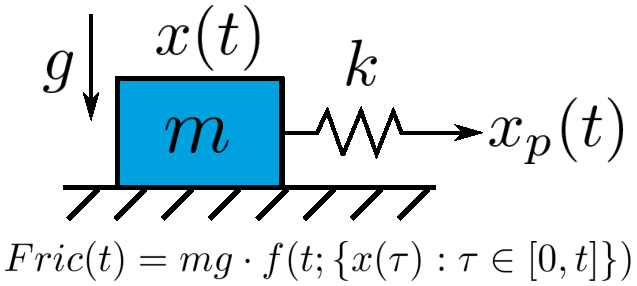
\includegraphics[width=0.4\textwidth]{SpringSlider.pdf}
    \caption{Example: spring slider under displacement-control driving force}
    \label{fig:springslider}
\end{figure}

In summary, 
by developing such a potential formulated friction, 
the implicit solving process of dynamic problems are turned into a convex optimization problem, 
which would guarantee us the existence of a unique solution for $(x_{n+1}, \bm{\xi}_{n+1})$. 
This would facilitate implicit solution which is usually difficult with the original rate-and-state friction. 
Since the original rate-and-state friction given by (\ref{eq:fRS}) is able to fit experimental data well with 4 parameters, 
it is crucial to verify that the potential-formulated friction specified by (\ref{eq:fpot}) can replicate rate-and-state friction sequences, 
with some selected $W, D^\dagger$ and $D$. 

In practice, 
it is useful to work with the dual formulation. 
Let $D^*(\bm{\dot{d}})$ be the Legendre transform of $D(\bm{\dot{\xi}})$, 
\begin{align}
    D^*\left(\dot{\bm{d}}\right) &= \sup_{\bm{\dot{\xi}} \in \mathbb{R}^d} \left\{\la \bm{\dot{d}}, \bm{\dot{\xi}} \ra -D(\dot{\bm{\xi}})\right\}. \label{eq:LegendreDstar}
\end{align} 
The advantage of using $D^*$ instead of $D$ is that instead of solving the non-linear equation for $\dot{\bm{\xi}}$ given by (\ref{eq:evolutionXi}), 
it is equivalent to computing $\dot{\bm{\xi}}$ by 
\begin{align}
    \dot{\bm{\xi}} &= \frac{d \Tilde{D}^*}{d \dot{\bm{d}}}\left(-\frac{\partial \Tilde{D}^\dagger}{\partial \bm{\xi}}\right) \label{eq:ComputeXiDot}, 
\end{align}
if $D\left(\bm{\dot{\xi}}\right)$ is convex in $\bm{\dot{\xi}}$. 


\section{Neural Network and training}
\label{sec:NN}
We use Neural Networks to approximate the above potentials within the deeping learning environment PyTorch \citep{paszke2019pytorch}, i.e., 
\begin{align}
    W(x) \approx W_{NN}(x; w_W), 
    D^\dagger(\dot{x}, \bm{\xi}) \approx D^\dagger_{NN}(\dot{x}, \bm{\xi}; w_{D^\dagger}), 
    D^*\left(\dot{\bm{d}}\right) \approx D^*_{NN}\left(\dot{\bm{d}}, w_{D^*}\right)\label{eq:NNpotentials},  
\end{align}
and we call the resulting architecture a Recurrent Neural Operator (RNO) following \citep{BurigedeEric2023, BurigedeMarkovian2023}. 

To find proper $W, D^\dagger$ and $D$ that give $f^{NN}$ similar enough to $f^{RS}$ under a set of rate-and-state parameters, 
we generate a synthetic dataset of $f^{RS}$'s by prescribing the slip histories $\{V = \dot{x}(t) : t \in [0, T]\}$. 
We then fit $f^{NN}$'s to $f^{RS}$'s by optimizing over the parameters of $W_{NN}, D^\dagger_{NN}$ and $D_{NN}$, 
as shown in Figure~\ref{fig:training}. 
\begin{figure}
    \centering
    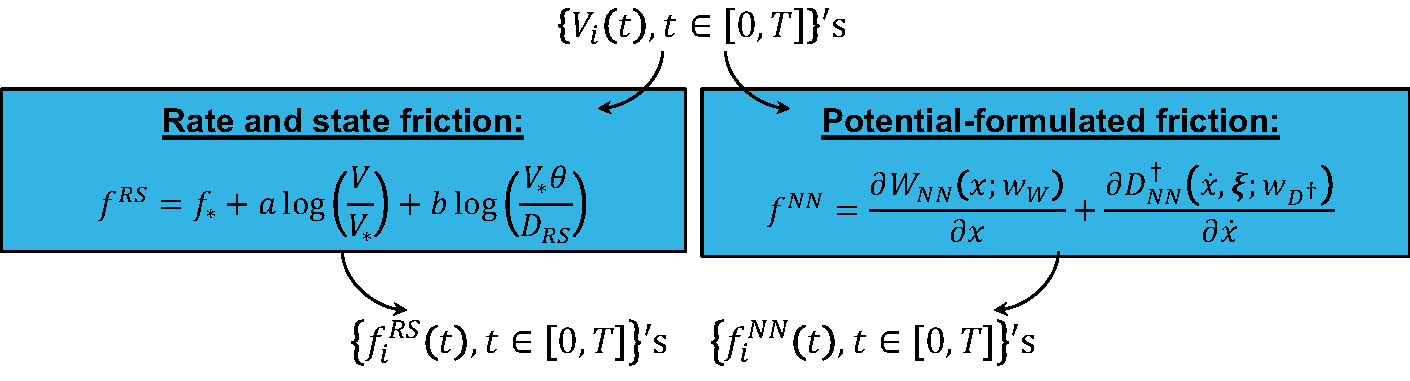
\includegraphics[width=0.8\textwidth]{training.pdf}
    \caption{Training of $W, D^\dagger$ and $D$ through fitting $f^{NN}$ to $f^{RS}$}
    \label{fig:training}
\end{figure}
And the loss function we use for training of the potentials is relative $L_p$ error, 
i.e., 
\begin{align}
    w_W^*, w_{D^\dagger}^*, w_D^* = \argmin_{w_W, w_{D^\dagger}, w_D} \frac{1}{N} \sum_{i=1}^N \frac{\|f^{NN}_i(t) - f^{RS}_i(t)\|_{L_p}}{\|f^{RS}_i(t)\|_{L_p}} \label{eq:relativeLpError}. 
\end{align}
In this study, 
the rate-and-state friction parameters are chosen to be 
\begin{align*}
    a &= 0.011, \\
    b &= 0.016, \\
    V_* &= 1\times 10^{-6}\ \mathrm{m/s}, \\
    D_{RS} &= 1\times10^{-8}\ \mathrm{m}, \\
    f_* &= 0.5109,  % f_* &= 0.58, 
\end{align*}
such that we do examine the ability of potential formulated friction to fit rate-weakening ($a - b < 0$) rate-and-state friction, 
which is more challenging to solve  numerically. 
Regarding the specific choices of $V_i(t)$'s, 
we take inspiration from both velocity jump tests for rate-and-state friction \citep{ruina_slip_1983}, 
as well as continuous variation sequences from the previous studies of RNO \citep{BurigedeEric2023, BurigedeMarkovian2023}. 
For the velocity jump sequences, 
$V_i(t)$'s are simple functions, 
i.e., the sum of a finite number of Heaviside functions, 
as shown by the first example in Figure~{\ref{fig:19thAnd99thRS}}. 
Note that the prescribed velocity jumps have to be on the log scale to cause significant changes in $f^{RS}$.  
While for the continuous variation sequences, 
$V_i(t)$'s vary continuously with $t$ and change their monotonicity at randomly-sampled times, 
as shown by the second example in Figure~\ref{fig:19thAnd99thRS}. 
The range of prescribed $V_i(t)$'s is set such that $V_{i}(t) / V_* \in [10^{-3}, 10^{1}]$ for both types of sequences. 
For easier plotting of displacements, 
we define 
\begin{align*}
    D_* = V_* \cdot 1\ \mathrm{s} = 1\times10^{-6}\ \mathrm{m}. 
\end{align*}

\begin{figure}
    \centering
    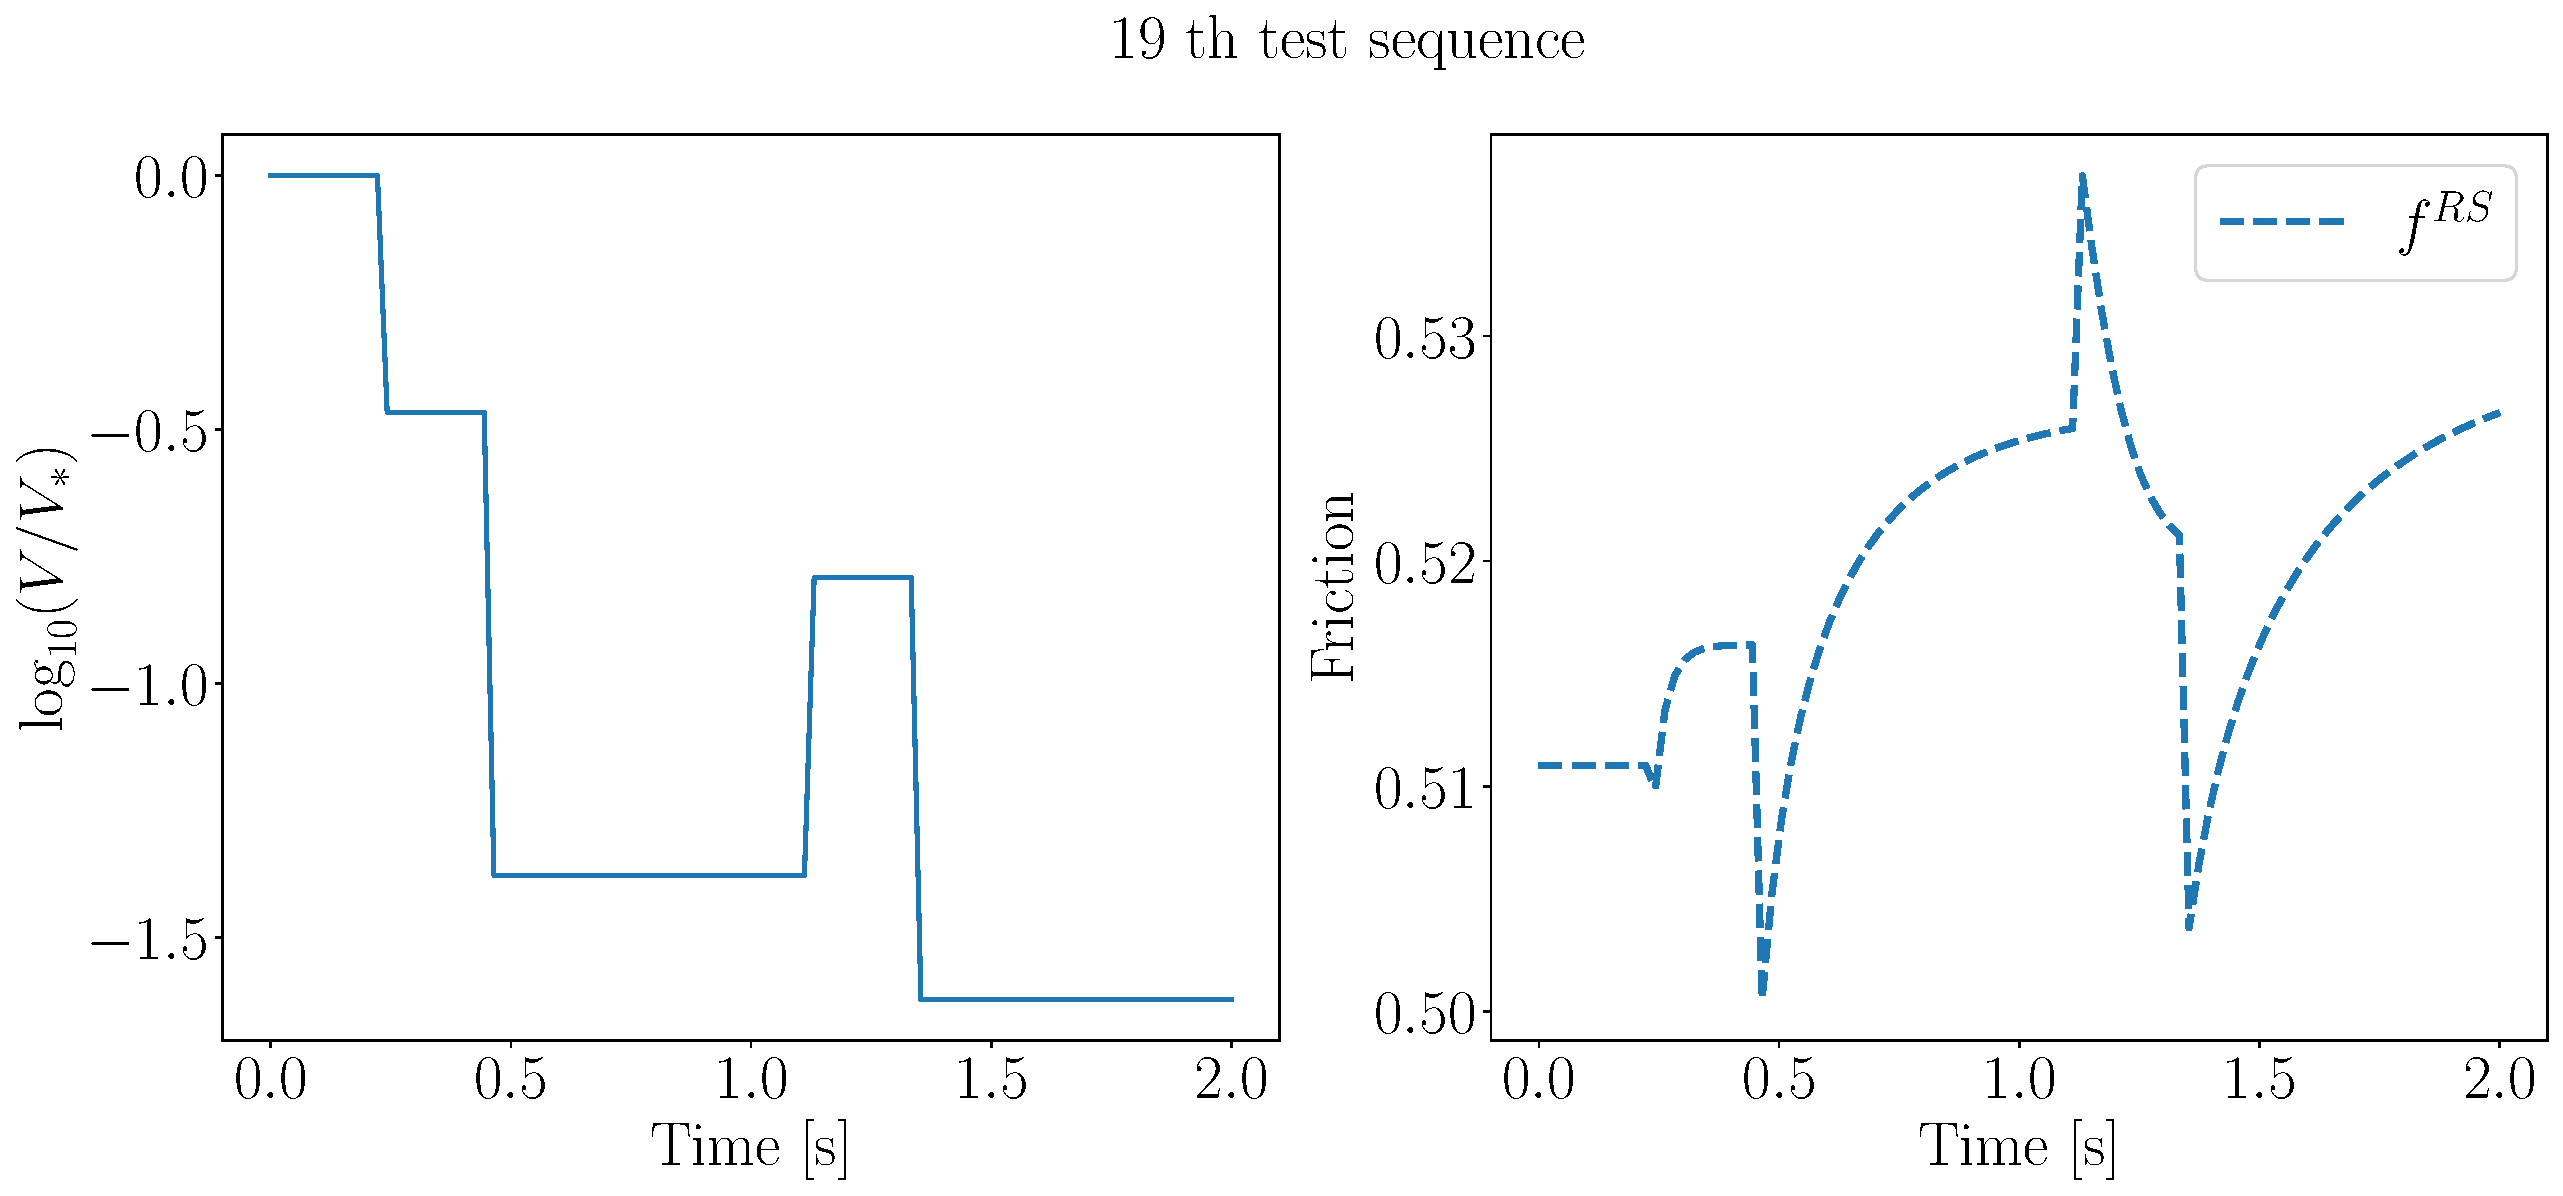
\includegraphics[height=0.3\textheight]{19thRS.pdf}
    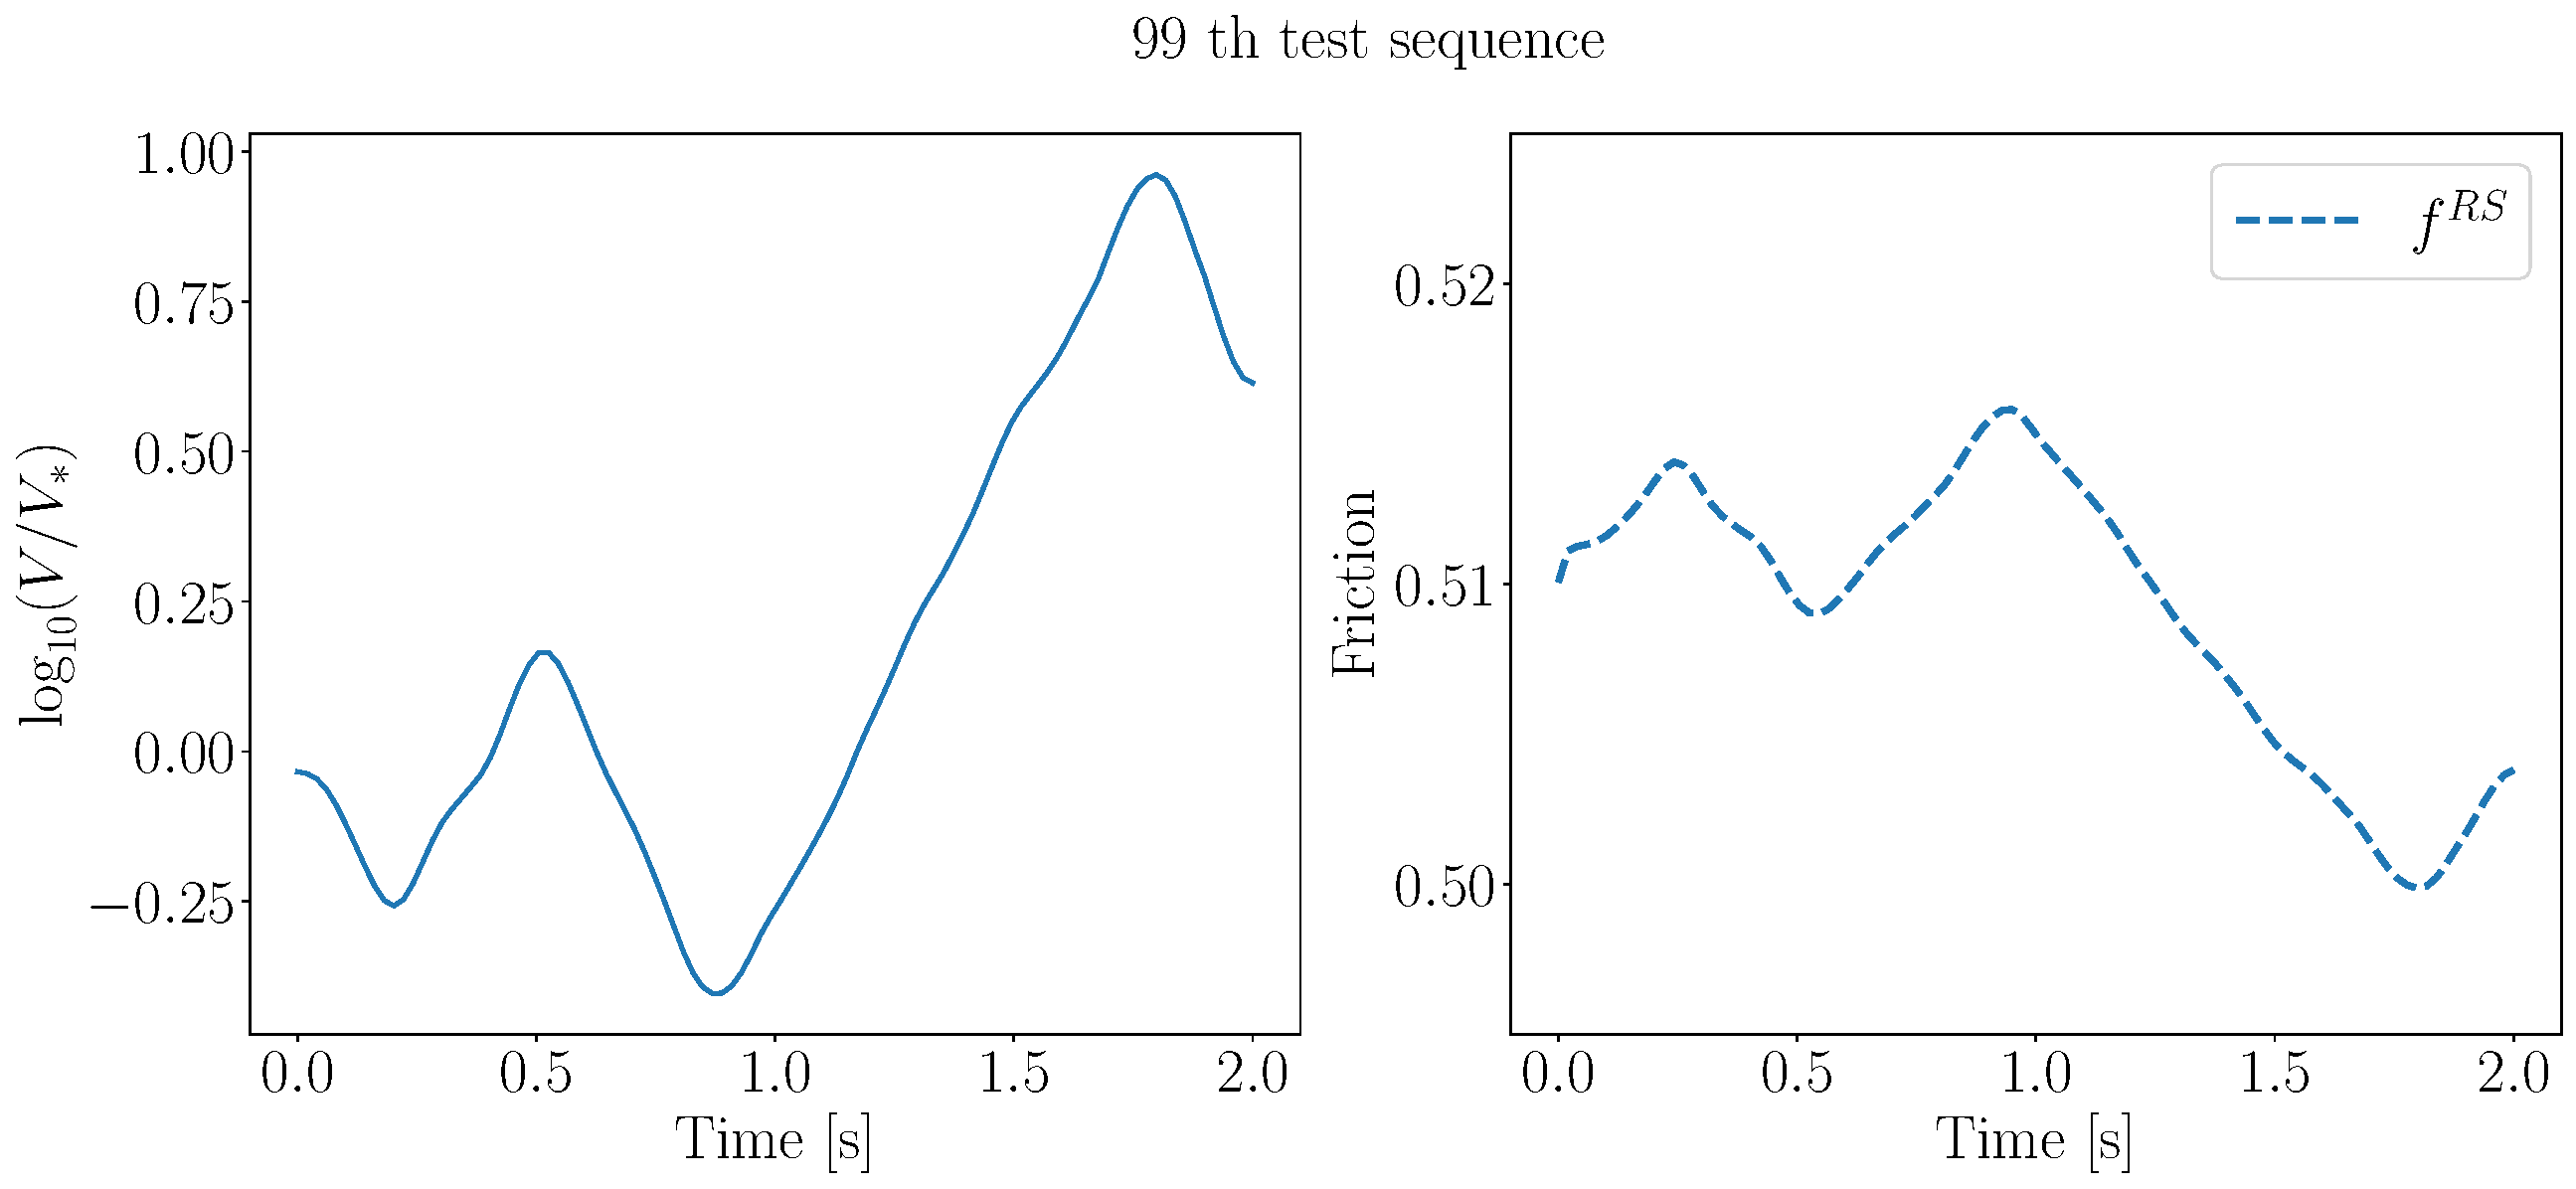
\includegraphics[height=0.3\textheight]{99thRS.pdf}
    \caption{Examples of velocity jump $V_i(t)$ (upper, sequence 19), 
    continuous variation $V_i(t)$ (lower, sequence 99) and their corresponding $f^{RS}$s in the synthetic dataset.}
    \label{fig:19thAnd99thRS}
\end{figure}

Within the training process, 
we apply Optuna \citep{akiba2019optuna} optimization package for hyper-parameter tuning of the Recurrent Neural Operators (RNO). 
Those hyper-parameters include learning rate, 
depth of the Neural Network, 
number of neurons within each layer, 
$p$ value for the $L_p$ norm, 
as well as the batch size in the training dataset. 
Detailed algorithm regarding the training process can be found in Algorithm~\ref{alg:TrainingOneEpoch}. 

\begin{algorithm}[htb!]
\caption{Training $W_{NN}(x; w_W), D_{NN}^\dagger(\dot{x}, \bm{\xi}; w_{D^\dagger})$ and $D_{NN}^*(\dot{\bm{d}}; w_D)$}\label{alg:TrainingOneEpoch}
\begin{algorithmic}
%% Setting parameters
% Input space
\Require training sequences $\left\{\dot{x}_i = V_{i}(t), f^{RS}_i(t) : t \in [0, T]\right\}_{i = 0}^N$.  
\Require $N_{epochs}$
%% Algorithm begins
\State $epoch = 0$
\While{$epoch<N_{epochs}$}
    \For {$i \in \{0, 1, ..., N\}$} \Comment{In practical sequences are passed in batches.}
        \State Fix $w_W$, $w_{D^\dagger}$, $w_D$
        \For {$n = 1, 2, ..., N^{(i)}$} \Comment{$N^{(i)}$ is number of time steps of sequence $i$. }
            \State $\xi_n \gets \xi_{n-1} + (t_n-t_{n-1}) \dot{\bm{\xi}}_{n-1}$
            \State $f^{NN}_n \gets \frac{\partial W_{NN}}{\partial x}(x_n) + \frac{\partial D^\dagger_NN}{\partial \dot{x}}(\dot{x}_n, \bm{\xi}_n)$
            \State \textcolor{red}{$\bm{\dot{\xi}}_n \gets $ solution of $\frac{d D_{NN}}{d \dot{\boldsymbol{\xi}}}(\dot{\bm{\xi}}) + \frac{\partial D_{NN}^\dagger}{\partial \boldsymbol{\xi}}(\dot{x}_n, \bm{\xi}_n) = 0$}
            \Comment{In practical $\dot{\bm{\xi}}_n = \frac{d D_{NN}^*}{d \dot{\bm{d}}}\left(-\frac{\partial D_{NN}^\dagger}{\partial \bm{\xi}}\left(\dot{x}_n, \bm{\xi}_n\right)\right)$}
        \EndFor
        \State Compute Loss $L(w_W, w_{D^\dagger}, w_D) = \|f^{RS} - f^{NN}(w_W, w_{D^\dagger}, w_D)\|_{{L}^p} / \|f^{RS}\|_{{L}^p}$
        \State Update $w_W, w_{D^\dagger}, w_D$ based on the gradient of $L$ w.r.t. $w_W, w_{D^\dagger}, w_D$
    \EndFor
    \State $epoch \gets epoch+1$
\EndWhile
\end{algorithmic}
\end{algorithm}
\section{Results and discussion}
\label{sec:resultsAndDiscussion}
In this section, 
we present how well the proposed RNO based potential formulated friction can fit the original rate-and-state friction, 
and also whether or not it facilitates implicit solution of dynamic problems through solving the spring slider example. 
\subsection{Fitting results to original rate-and-state friction}
After 100 epochs of training under the optimal Neural Network structure given by OPTUNA, 
the RNO potentials are able to fit the original rate-and-state sequences well. 
Figure~\ref{fig:19thAnd99thRSNN} shows the fitting results of the two example sequences early mentioned in Figure~\ref{fig:19thAnd99thRS}. 
Note that these two sequences are in the test dataset and have not been used for training the potentials. 
After training of the potentials $W_{NN}, D^\dagger_{NN}$ and $D^*_{NN}$, 
we can obtain $f^{NN}$s that are fairly close to $f^{RS}$s. 
Table~\ref{tab:dimXi} confirms that the error between $f^{NN}$ and $f^{RS}$ is small, 
and that there needs to be at least $1$ hidden variable ($\dim(\bm{\xi})$) to achieve small error. 
Since further increasing the number of hidden variables does not reduce the error, 
the results shown next are all based on $\dim(\bm{\xi}) = 1$. 
The fact that it suffices to use $\dim(\bm{\xi}) = 1$ makes intuitive sense since the original rate-and-state friction has only one state variable $\theta$. 

Due to limited access to experimental data with the same rate-and-state friction properties, 
we cannot compare the error of $f^{RS}$ and $f^{NN}$ both fitted to 
experimental sequences $f^{EXP}$. 
We here include a typical rate-and-state fitted experimental sequence from (Kim et al., in preparation, 2024), 
which is shown by Figure~\ref{fig:RSVsExp}. 
The best fit rate-and-state sequence achieves an relative $L_2$ error of $0.0268$, 
which is two orders of magnitude higher than the average relative $L_2$ of fitting $f^{NN}$ to $f^{RS}$. 
This implies that the fitting error between $f^{NN}$ and $f^{RS}$ is negligible compared with fitting $f^{RS}$ to noisier $f^{EXP}$, 
and thus $f^{NN}$ has comparable ability to explain the history dependencies in the empirical observations. 

\begin{figure}[htbp]
    \centering
    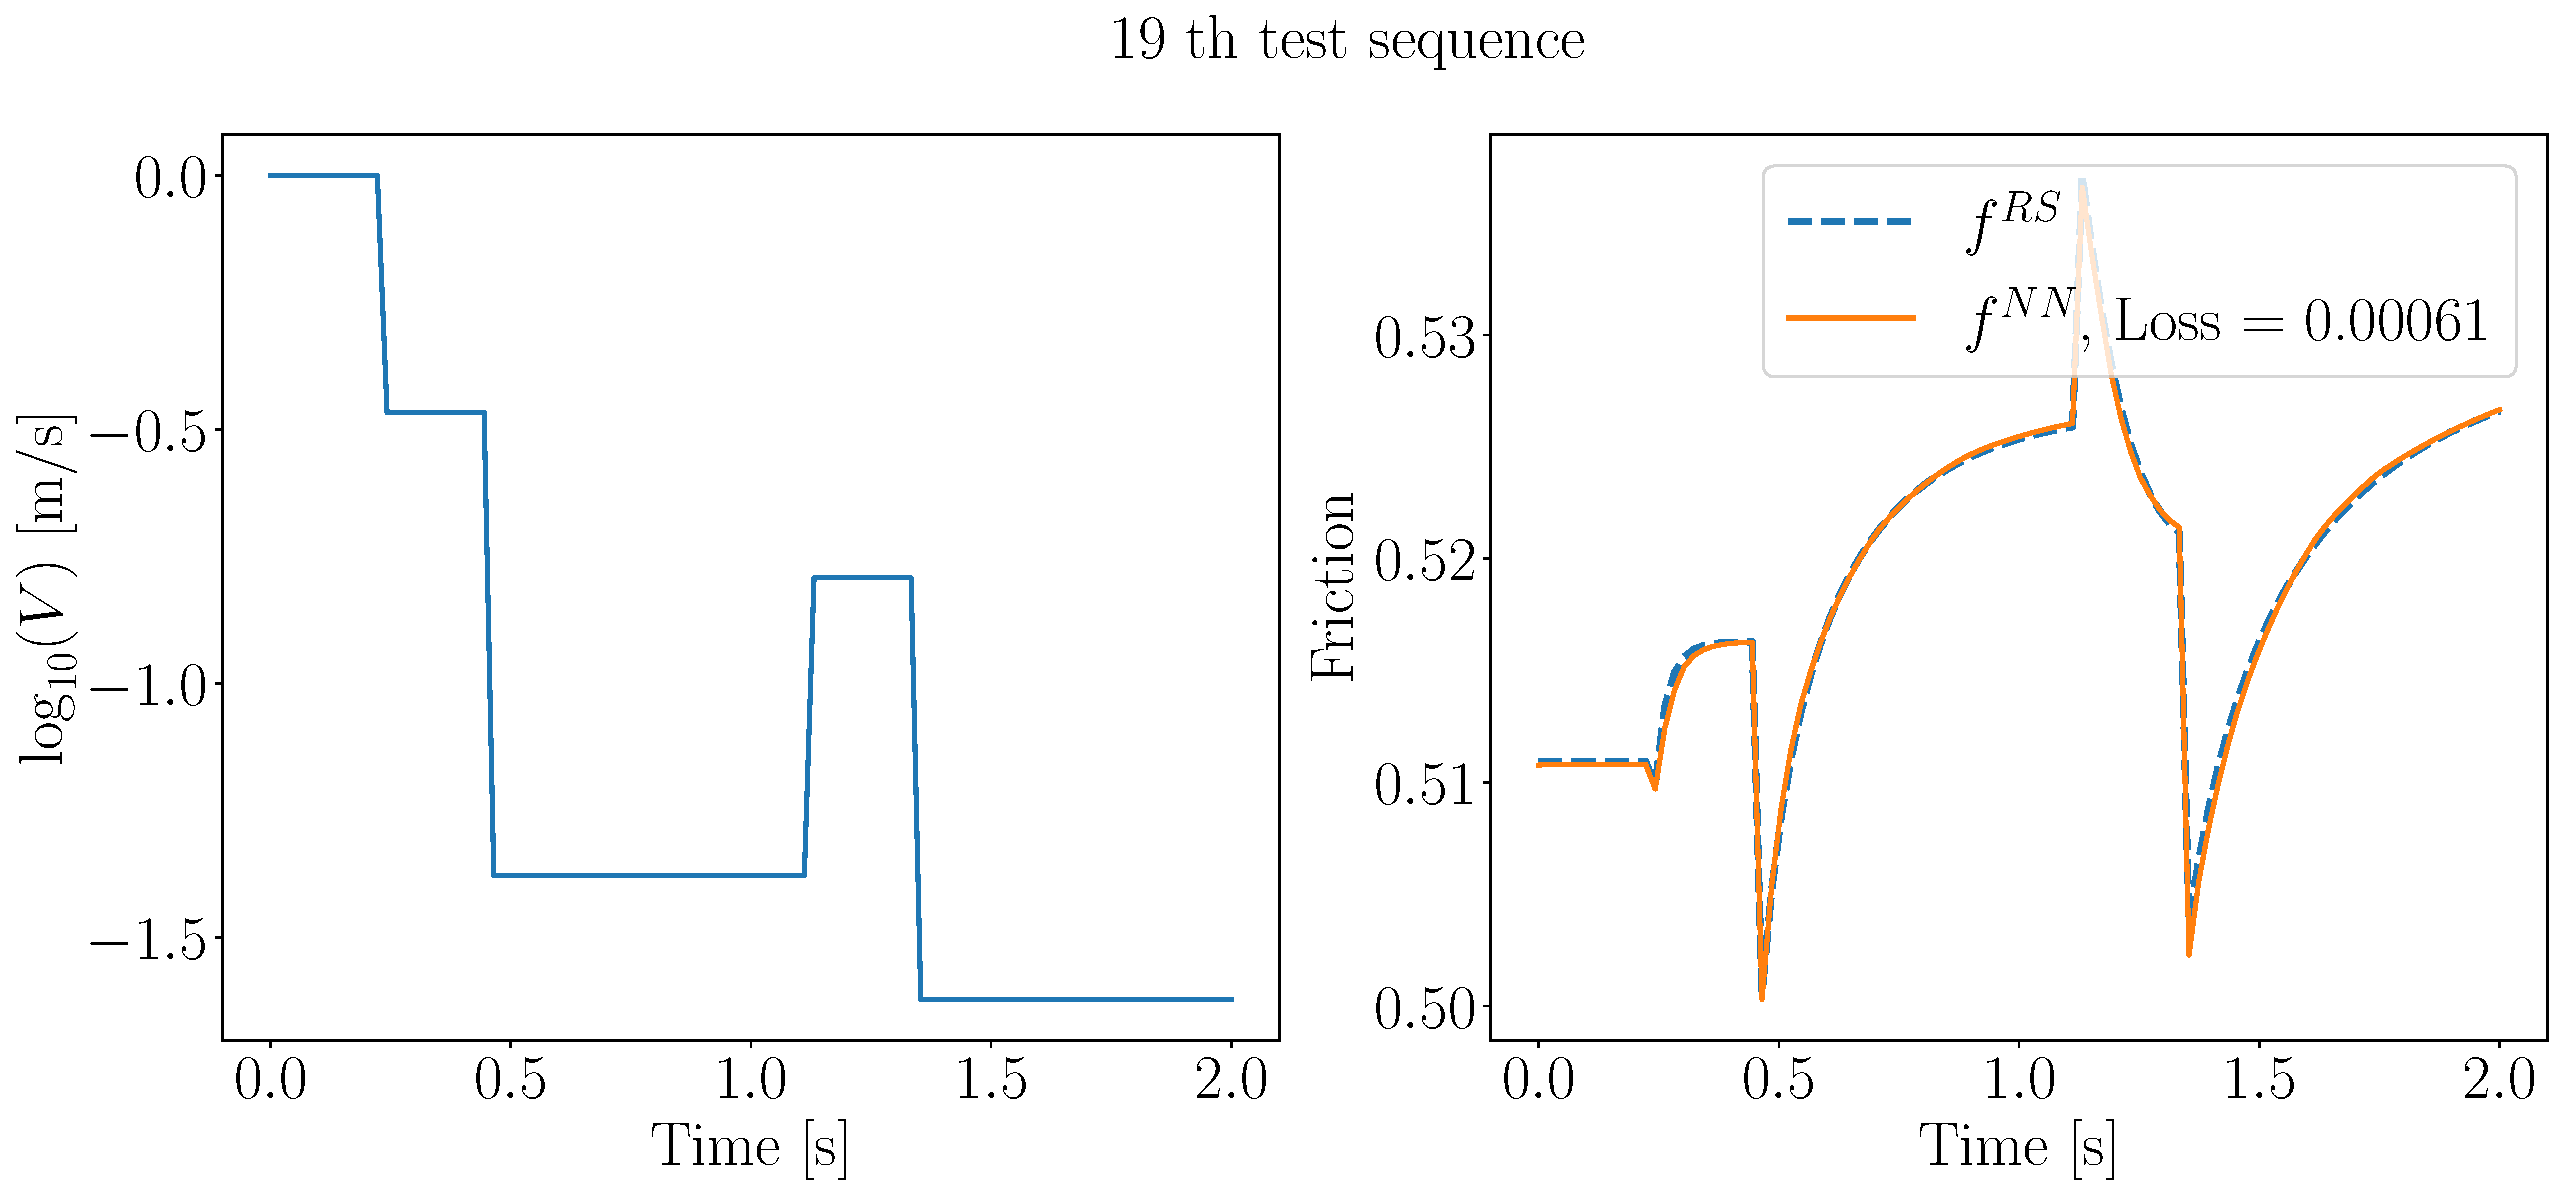
\includegraphics[height=0.3\textheight]{figures/19thRSNN.pdf}
    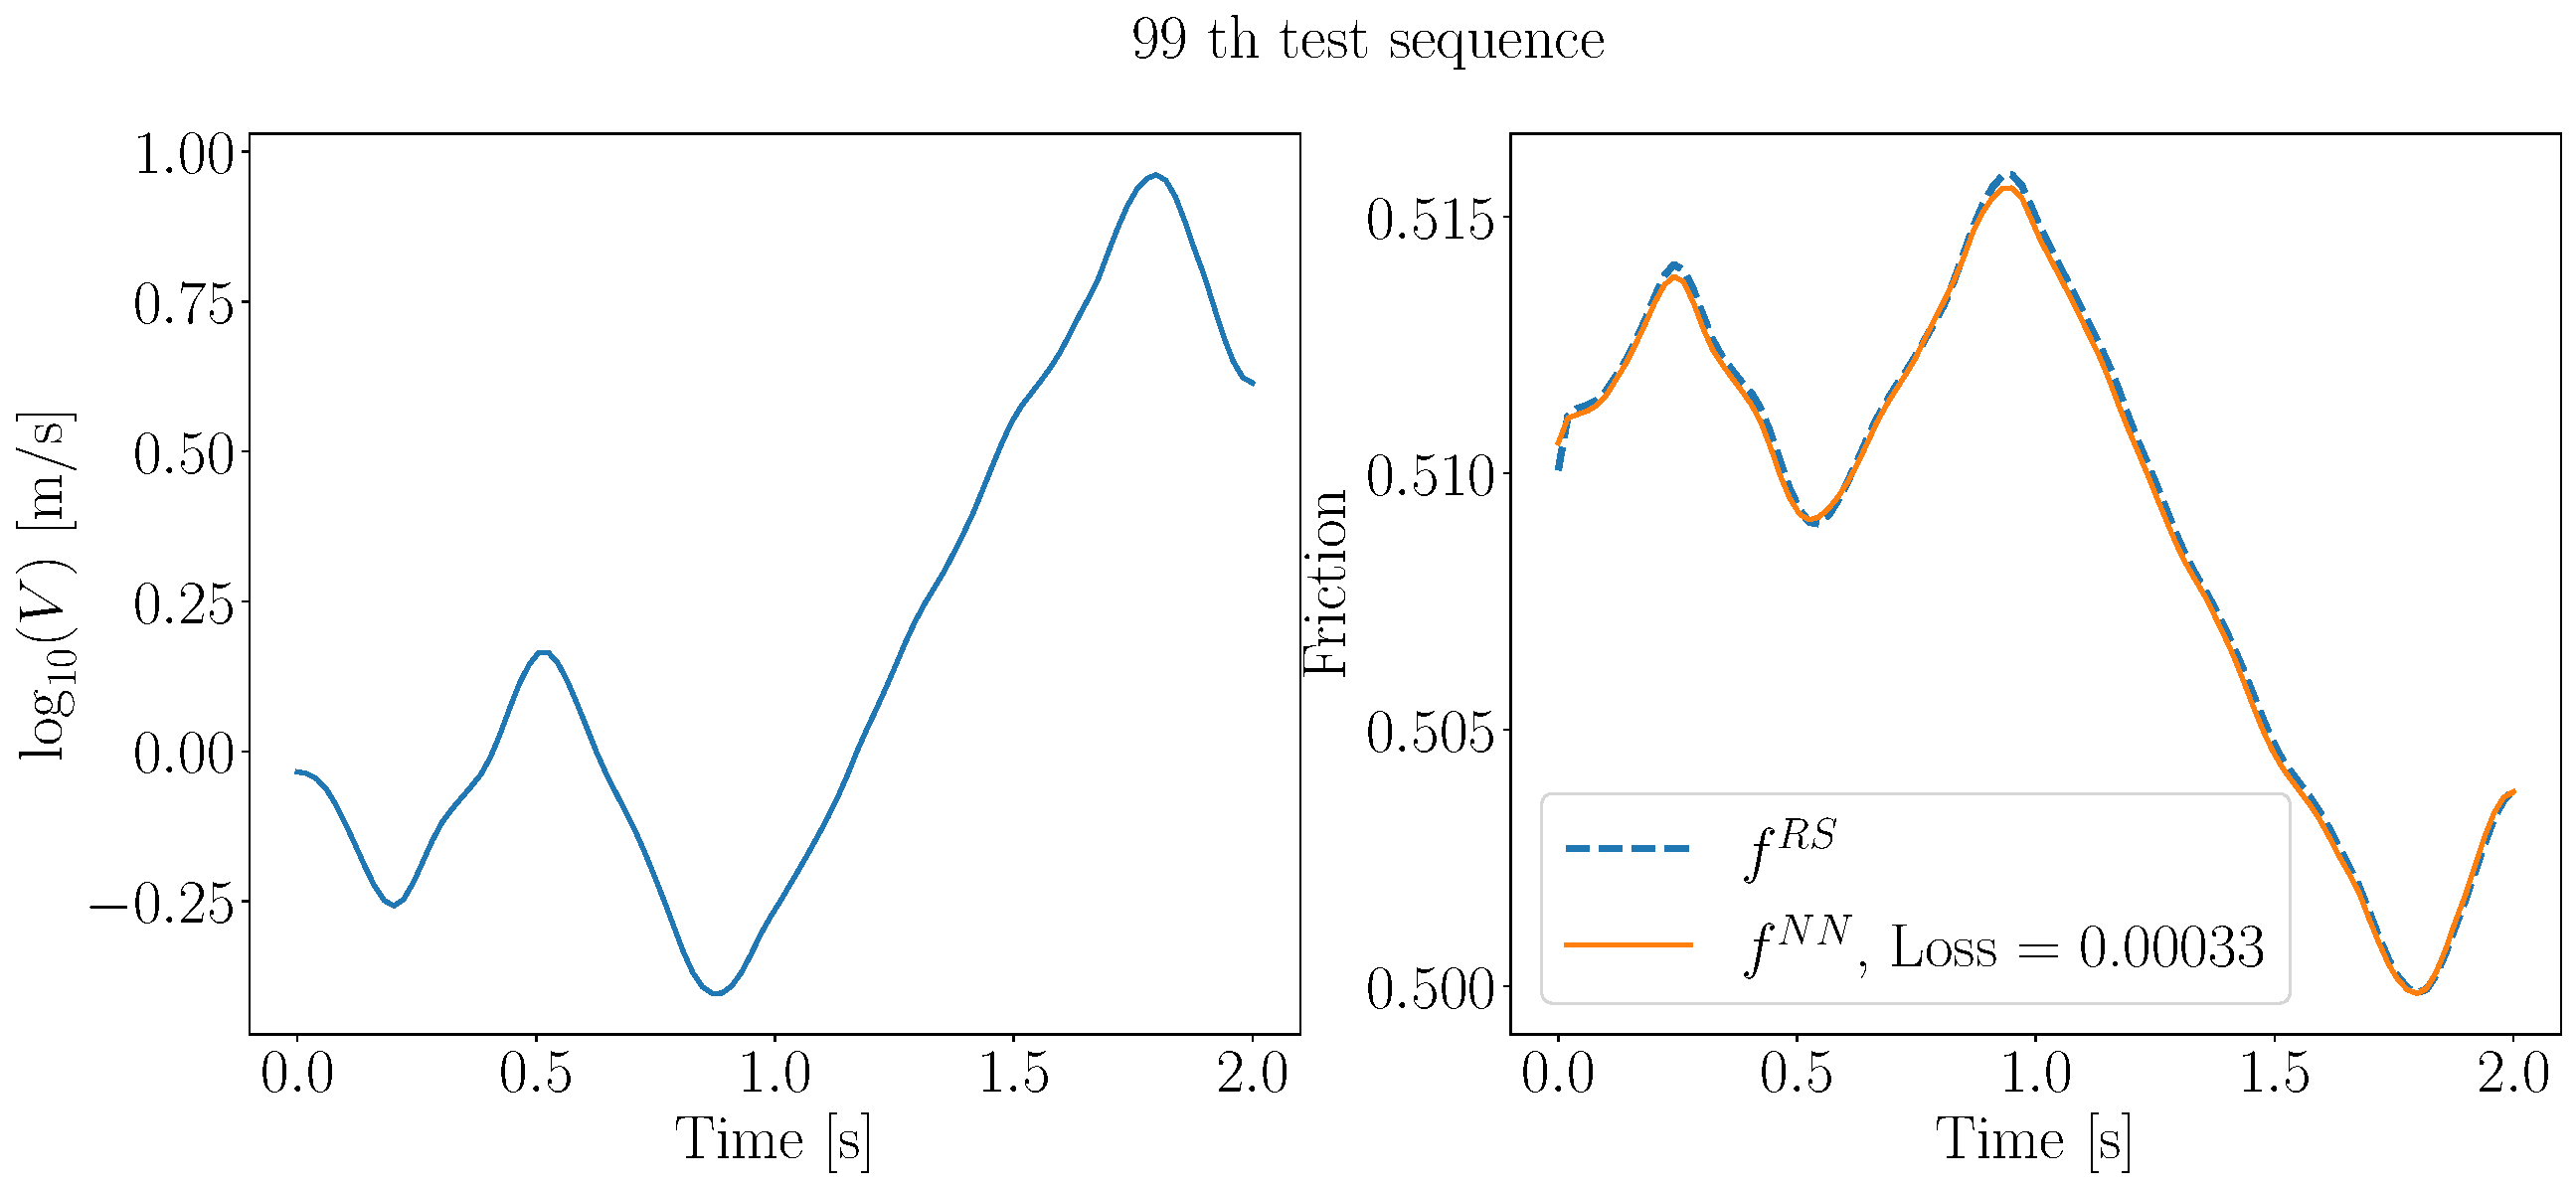
\includegraphics[height=0.3\textheight]{figures/99thRSNN.pdf}
    \caption{Examples of trained $f^{NN}$ vs. $f^{RS}$ for both velocity jump (upper) and continuous variation (lower) sequences. 
    Loss here refers to relative $L_2$ error as defined by (\ref{eq:relativeLpError}). 
    These two sequences are from the test dataset and are not used for training the potentials.}
    \label{fig:19thAnd99thRSNN}
\end{figure}

\begin{figure}[htbp]
    \centering
    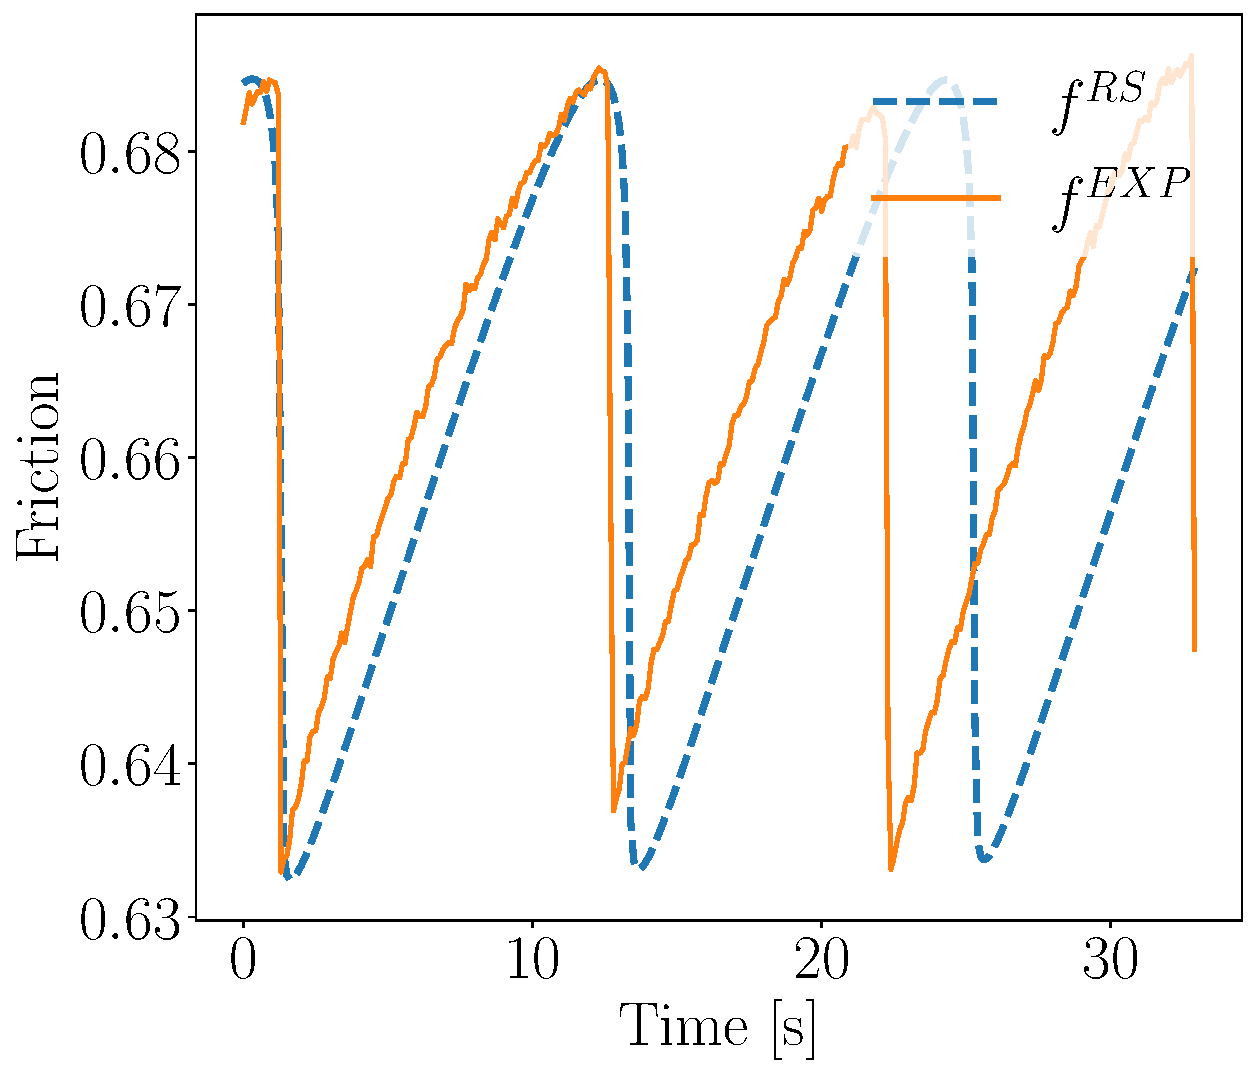
\includegraphics[width=0.4\textwidth]{figures/RSVsExp.pdf}
    \caption{A typical fit of rate-and-state friction to experimental data, 
    the relative $L_2$ error of $f^{RS}$ against $f^{EXP}$ is 0.0268. 
    Data provided by Taeho Kim.}
    \label{fig:RSVsExp}
\end{figure}

\begin{table}[htbp]
    \centering
    \begin{tabular}{cccc}
        \hline
        $\dim(\bm{\xi})$ & 0 & 1 & 2 \\
        \hline
        Training error ($L_2$) & 0.18 $\pm$ 0.01 & 0.0004 $\pm$ 0.0004 & 0.0007 $\pm$ 0.0006\\
        Testing error ($L_2$) & 0.18 $\pm$ 0.01 & 0.0005 $\pm$ 0.0004 & 0.0007 $\pm$ 0.0006 \\
        \hline
    \end{tabular}
    \caption{Training and testing relative $L_2$ error for $\dim(\bm{\xi}) = 0, 1, 2$, 
    averaged over 160 test sequences. 
    Error decreases significantly after introducing one hidden variable $\dim(\bm{\xi}) = 1$, 
    while introducing more hidden variables do not further reduce the error. }
    \label{tab:dimXi}
\end{table}

\subsection{The trained potentials $W, D^\dagger$ and $D^*$}
To make (\ref{eq:JfunctionalMin}) a convex minimization problem, 
we need to confirm convexity of $J$ in $(x, \xi)$. 
Figure~\ref{fig:WAndD} shows that the learnt $W$ is linear in $x$, 
and thus also convex. 
The fact that $W$ is linear makes sense because of material frame indifference.   
$D^*$ is convex in $\dot{d}$, 
which is consistent with its definition as the Legendre transform of $D$. 
Figure~\ref{fig:Ddagger} plots $D^\dagger(\dot{x}, \xi)$, 
and it is not convex because $\partial^2 D^\dagger / \partial \dot{x}^2 < 0$. 
To ensure convexity of $J$ in $(x, \xi)$, 
we need the Hessian of $J$ to be positive semi-definite for all $(x, \xi)$, 
which ends up posing a constraint on $\Delta t$: 
\begin{align}
    &1 \cdot m + \Delta t \left(\frac{\partial^2 D^\dagger}{\partial \dot{x}^2}\right) + O(\Delta t^2)  &\ge 0, \label{eq:PSD1}\\
    & 1 \cdot m \frac{d^2D}{d\dot{\xi}^2} 
    + \Delta t \left(\frac{\partial^2 D^\dagger}{\partial \dot{x}^2} \frac{d^2D}{d\dot{\xi}^2} + m \frac{\partial^2 D^\dagger}{\partial \xi^2}\right) 
    &\notag \\
    & + \Delta t^2 \left[\left(k + \frac{d^2W}{dx^2}\right)\frac{d^2D}{d\dot{\xi}^2} + \frac{\partial^2 D^\dagger}{\partial \dot{x}^2}\frac{\partial^2 D^\dagger}{\partial \xi^2}-\frac{\partial^2D^\dagger}{\partial \dot{x} \partial \xi}\right] 
    &\notag \\
    & + \Delta t^3 \left[\left(k + \frac{d^2W}{dx^2}\right)\frac{\partial^2D^\dagger}{\partial \xi^2}\right] & \ge 0. \label{eq:PSD2}
\end{align}

Equation (\ref{eq:PSD1}) can be satisfied with $\Delta t$ smaller than an upper bound, 
since then the $m$ term will dominate even if $\partial^2 D^\dagger / \partial \dot{x}^2 < 0$. 
(\ref{eq:PSD2}) also reduces to an upper bound constraint on $\Delta t$, 
since $d^2 D / d \dot{\xi}^2 > 0$ based on the assumption. 
In practical it is also convex because it is the Legendre transform of the learnt $D^*(\dot{d})$. 


\begin{figure}[htbp]
    \centering
    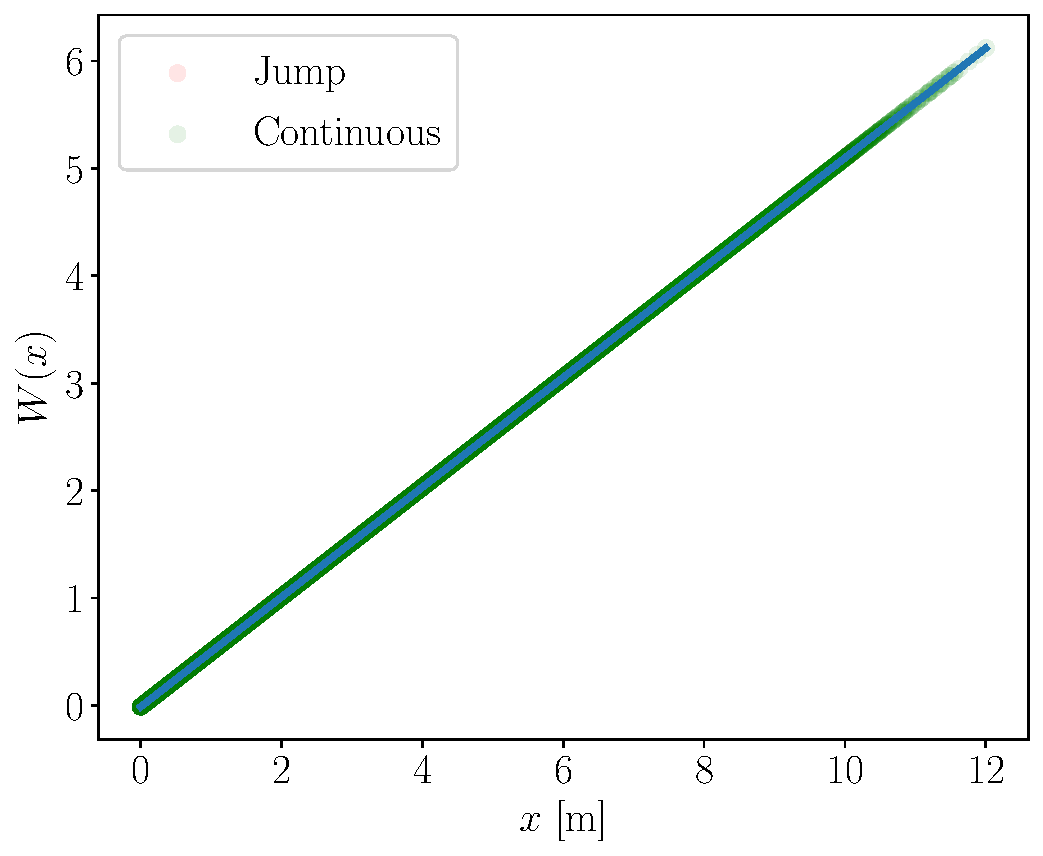
\includegraphics[height=0.25\textheight]{figures/Trial0216_combined_800_W.pdf}
    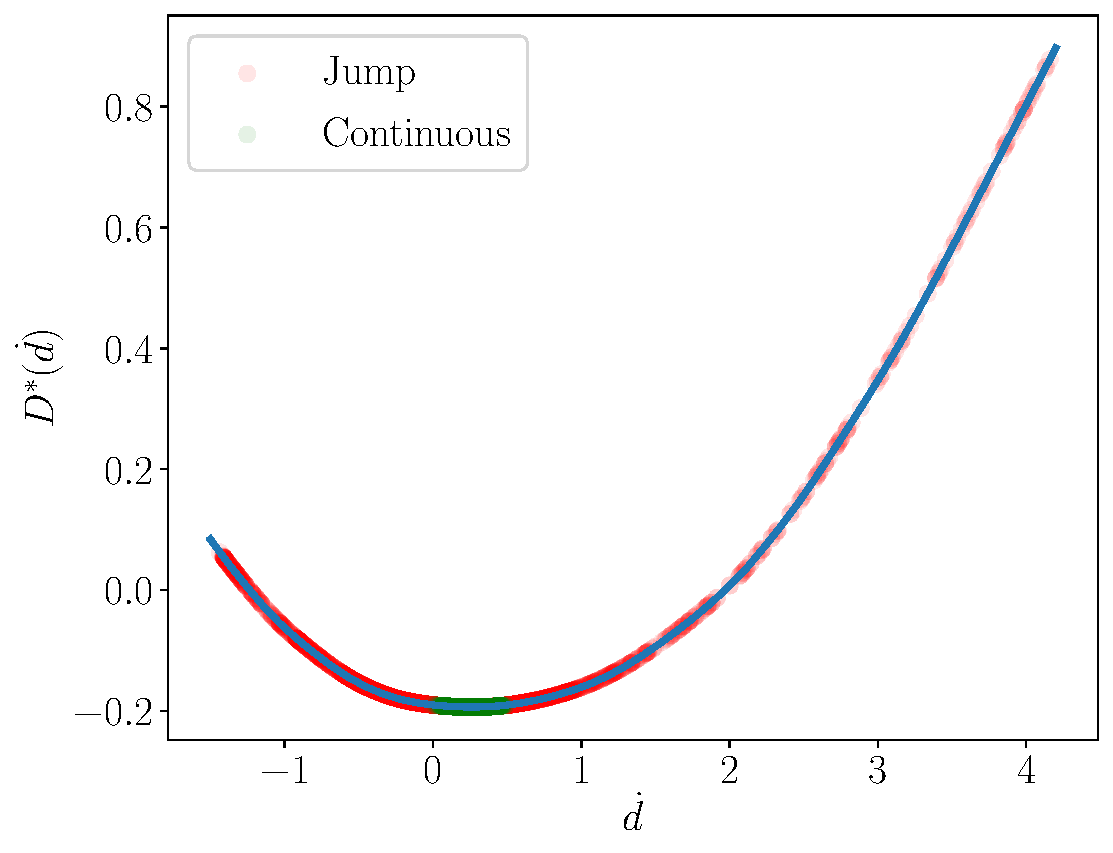
\includegraphics[height=0.25\textheight]{figures/Trial0216_combined_800_D_star.pdf}
    \caption{Learnt $W(x)$ (left) and $D^*(\dot{d})$ (right). 
    $W$ is linear in $x$ corresponding to the reference friction coefficient, 
    $D^*$ is convex, 
    which complies with the definition as the Legendre transform of $D$.}
    \label{fig:WAndD}
\end{figure}
\begin{figure}[htbp]
    \centering
    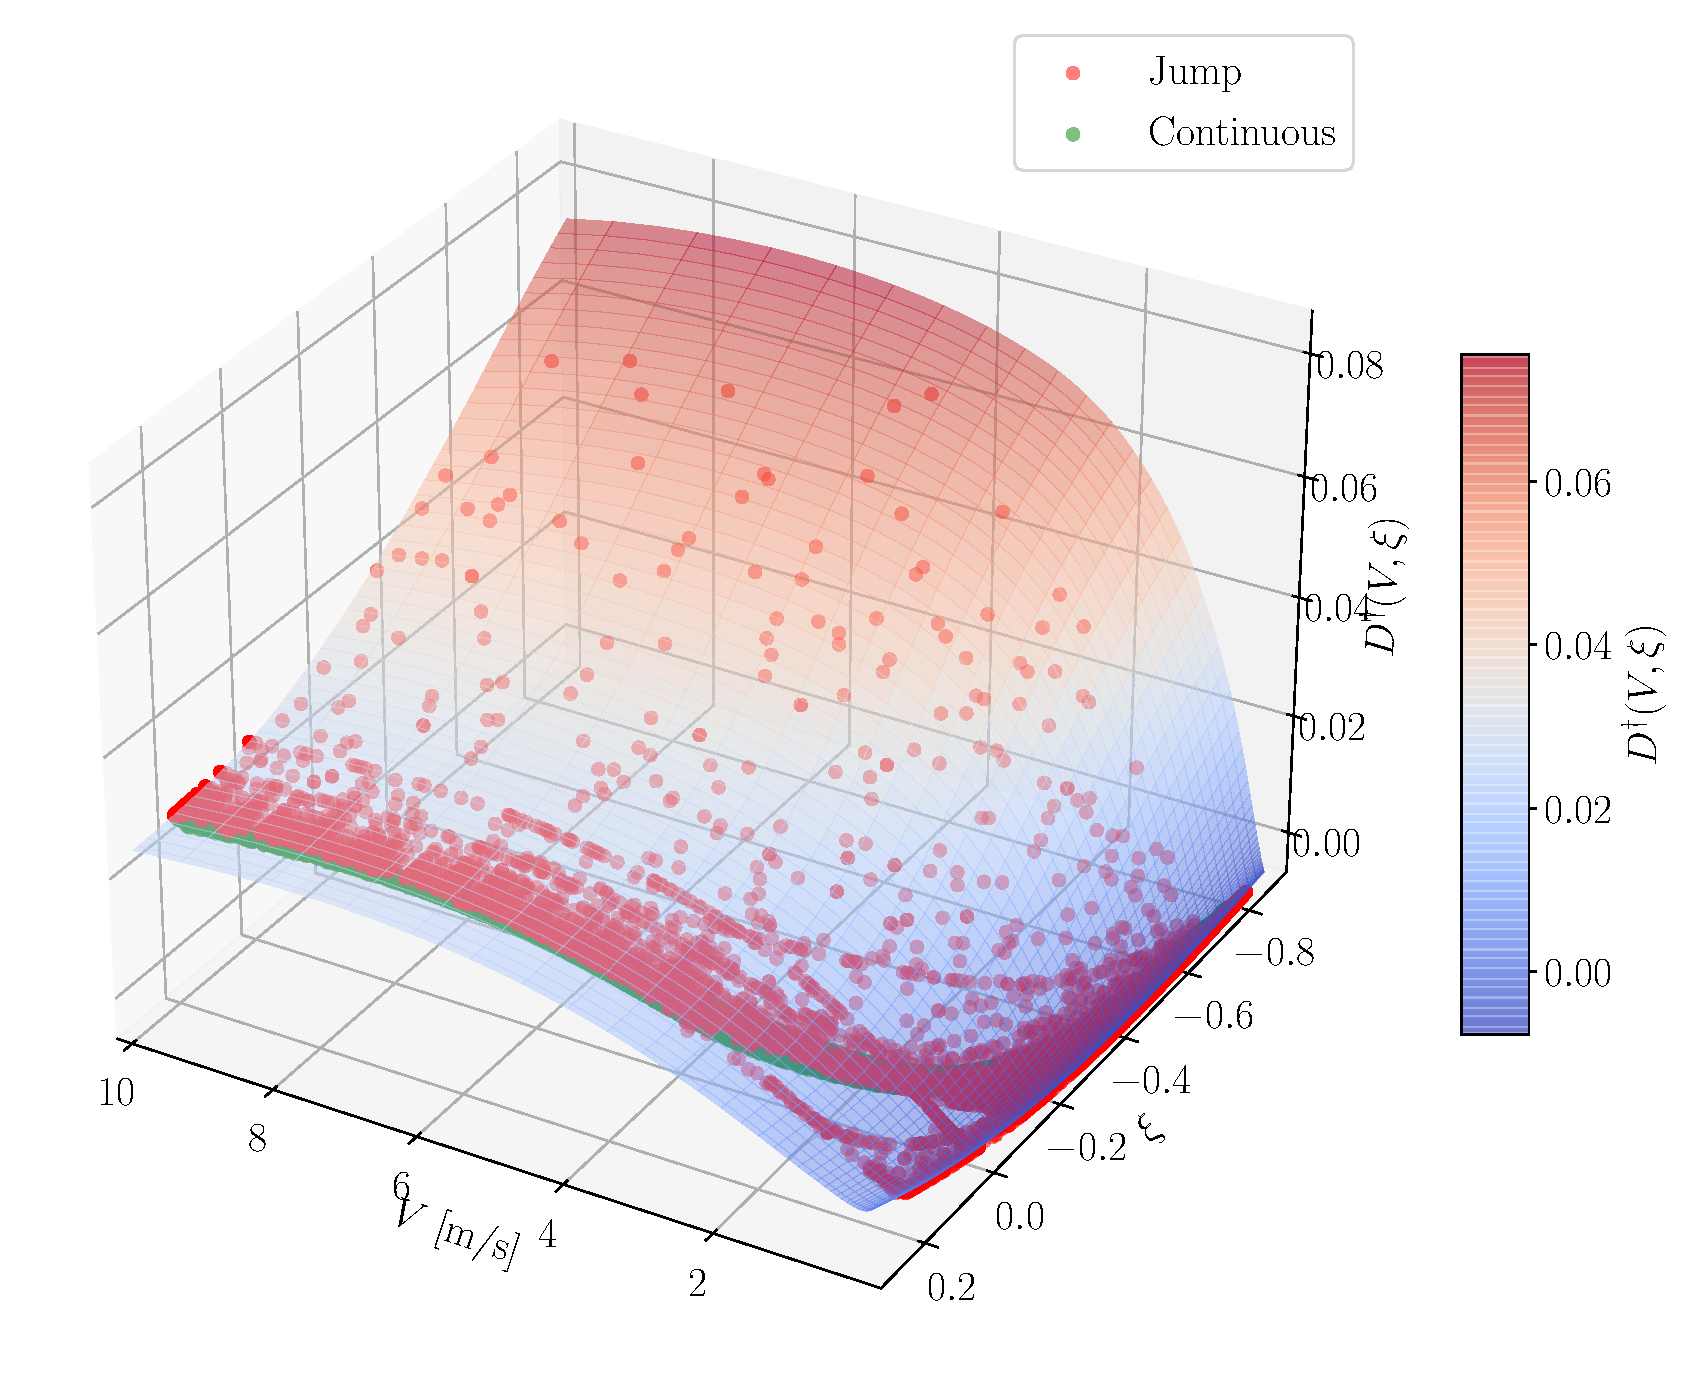
\includegraphics[height=0.5\textheight]{figures/Trial0216_combined_800_D_dagger_normal.pdf}
    \caption{Learnt $D^\dagger(\dot{x}, \bm{\xi})$, 
    $D^\dagger$ is not convex in $(\dot{x}, \xi)$.
    The red dots show the trajectories of velocity-jump dataset, 
    while the green dots show the trajectories of continuous variation dataset.}
    \label{fig:Ddagger}
\end{figure}

In summary, 
we find that of the three learnt potentials, 
$W$ is linear in $x$, 
consistent with material-frame indifference; 
$D^*$ is convex in $\dot{d}$, 
consistent with its definition by Legendre transform; 
while $D^\dagger$ is not convex in $(\dot{x}, \xi)$. 
However, 
one can still achieve convexity of $J(x, \xi)$ in (\ref{eq:Jfunctional}) with an upper bound constraint on $\Delta t$, 
and thus it is legitimate to write (\ref{eq:JfunctionalMin}) as a convex minimization problem. 

\subsection{Uniqueness of the hidden variable $\xi$}
One important property of the hidden variable $\xi$ is that since we cannot attach a concrete physical meaning to it, 
it is possibly non-unique. 
In practice, 
even different training runs can possibly lead to different $\xi$'s that all fit the training dataset well. 
However, 
in our potential formulation an underlying assumption is that $D$ is only a function of $\dot{\xi}$. 
Then if there exists $\eta = f(\xi)$ as a different hidden variable with $f$ and $f^{-1}$ being smooth, 
we have 
\begin{align}
    D^\eta\left(\dot{\eta}\right) = D^\eta\left(f'(\xi)\dot{\xi}\right) = D^\xi \left(\dot{\xi}\right) \label{eq:uniqueXi}, 
\end{align}
which implies that $f'(\xi)$ is a constant, 
and thus $\xi$ is unique up to affine transformations. 

We verify the above-discussed uniqueness of $\xi$ by training three different models on three datasets generated similarly using the same rate-and-state friction model. 
Then we obtain the trajectories of $\xi$s of the three trained model on the same test dataset. 
After performing linear regression of $\xi^{(3)}$ and $\xi^{(2)}$s on $\xi^{(1)}$, 
i.e. the hidden variable from the first trained model, 
we check their regression coefficient as a reflection of how linearly correlated the $\xi$s are. 

\begin{figure}[htbp]
    \centering
    \includegraphics[width=0.9\textwidth]{figures/nonuniqueXis.pdf}
    \caption{Linear regression of $\xi^{(3)}$ and $\xi^{(2)}$s on $\xi^{(1)}$. 
    Red and green dots are the data points while the solid lines are the regression result.
    $(0, 0)$ should be a fixed point since all sequences start with $\xi = 0$ as their initial condition.}
    \label{fig:nonuniqueXis}
\end{figure}

Figure~\ref{fig:nonuniqueXis} shows that the regression coefficient is $>0.98$ and thus the different $\xi$s are indeed unique up to linear transform.


\subsection{Example: solving spring slider under displacement control loading}
As stated above, 
the potential formulated friction should facilitate implicit solution of dynamic initial value problems, 
because advancing the solution to the next time step can be written as a convex minimization problem given by (\ref{eq:JfunctionalMin}). 
Here we try to verify that by considering the spring-slider problem with displacement-control loading. 
As shown by Figure~\ref{fig:springslider}, 
friction between the mass block and the ground is modeled with either original rate-and-state friction or trained potentials with the same rate-and-state properties. 
We testify the two friction formulations with both explicit (4th order Runge Kutta) and implicit (Adams) solvers trying to solve the same spring-slider problem. 
The solvers are imported from a standard ODE solver package torchdiffeq \cite{torchdiffeq}.
Spring constant $k$ is randomly sampled within a range that covers both $k < k_{crit}$ and $k > k_{crit}$, 
where $k_{crit}$ is the critical stiffness for unstable stick-slip events to happen under constant loading speed $\dot{x}_p(t)$ \cite{rice_stability_1983, Gu_Rice_1984}. 
and we create a dataset of 77 loading sequences with different velocity-jump-like $x_p(t)$s. 

We first notice that since the training dataset of the potentials does not include these spring-slider sequences of $V(t), f(t)$, 
the error between the potential friction and
the original rate-and-state friction is large. 
To resolve this, 
we generate $200$ sequences from solving the spring-slider problem with rate-and-state friction and different loadings, 
and further train our potentials on these $200$ sequences for $400$ epochs. 
Indeed the further-trained NN potentials (denoted as NN') reduce the error between $f^{NN'}$ and $f^{RS}$ when solving spring-slider sequences. 

Table~\ref{tab:NNvsNNPrime} shows that after further training the potentials on spring-slider solutions by rate-and-state friction, 
the relative $L_2$ error on $x(t), \dot{x}(t), f(t)$ decreases by more than $50\%$. 
Figure~\ref{fig:SSseq8} plots an example spring-slider sequence. 
It is clear that further trained NN' agrees better with the solution obtained by the original rate-and-state friction. 
Another example sequence is shown by Figure~\ref{fig:SSseq9}.
The results and discussions next will all be based on the solution of NN'. 

\begin{figure}[htbp]
    \centering
    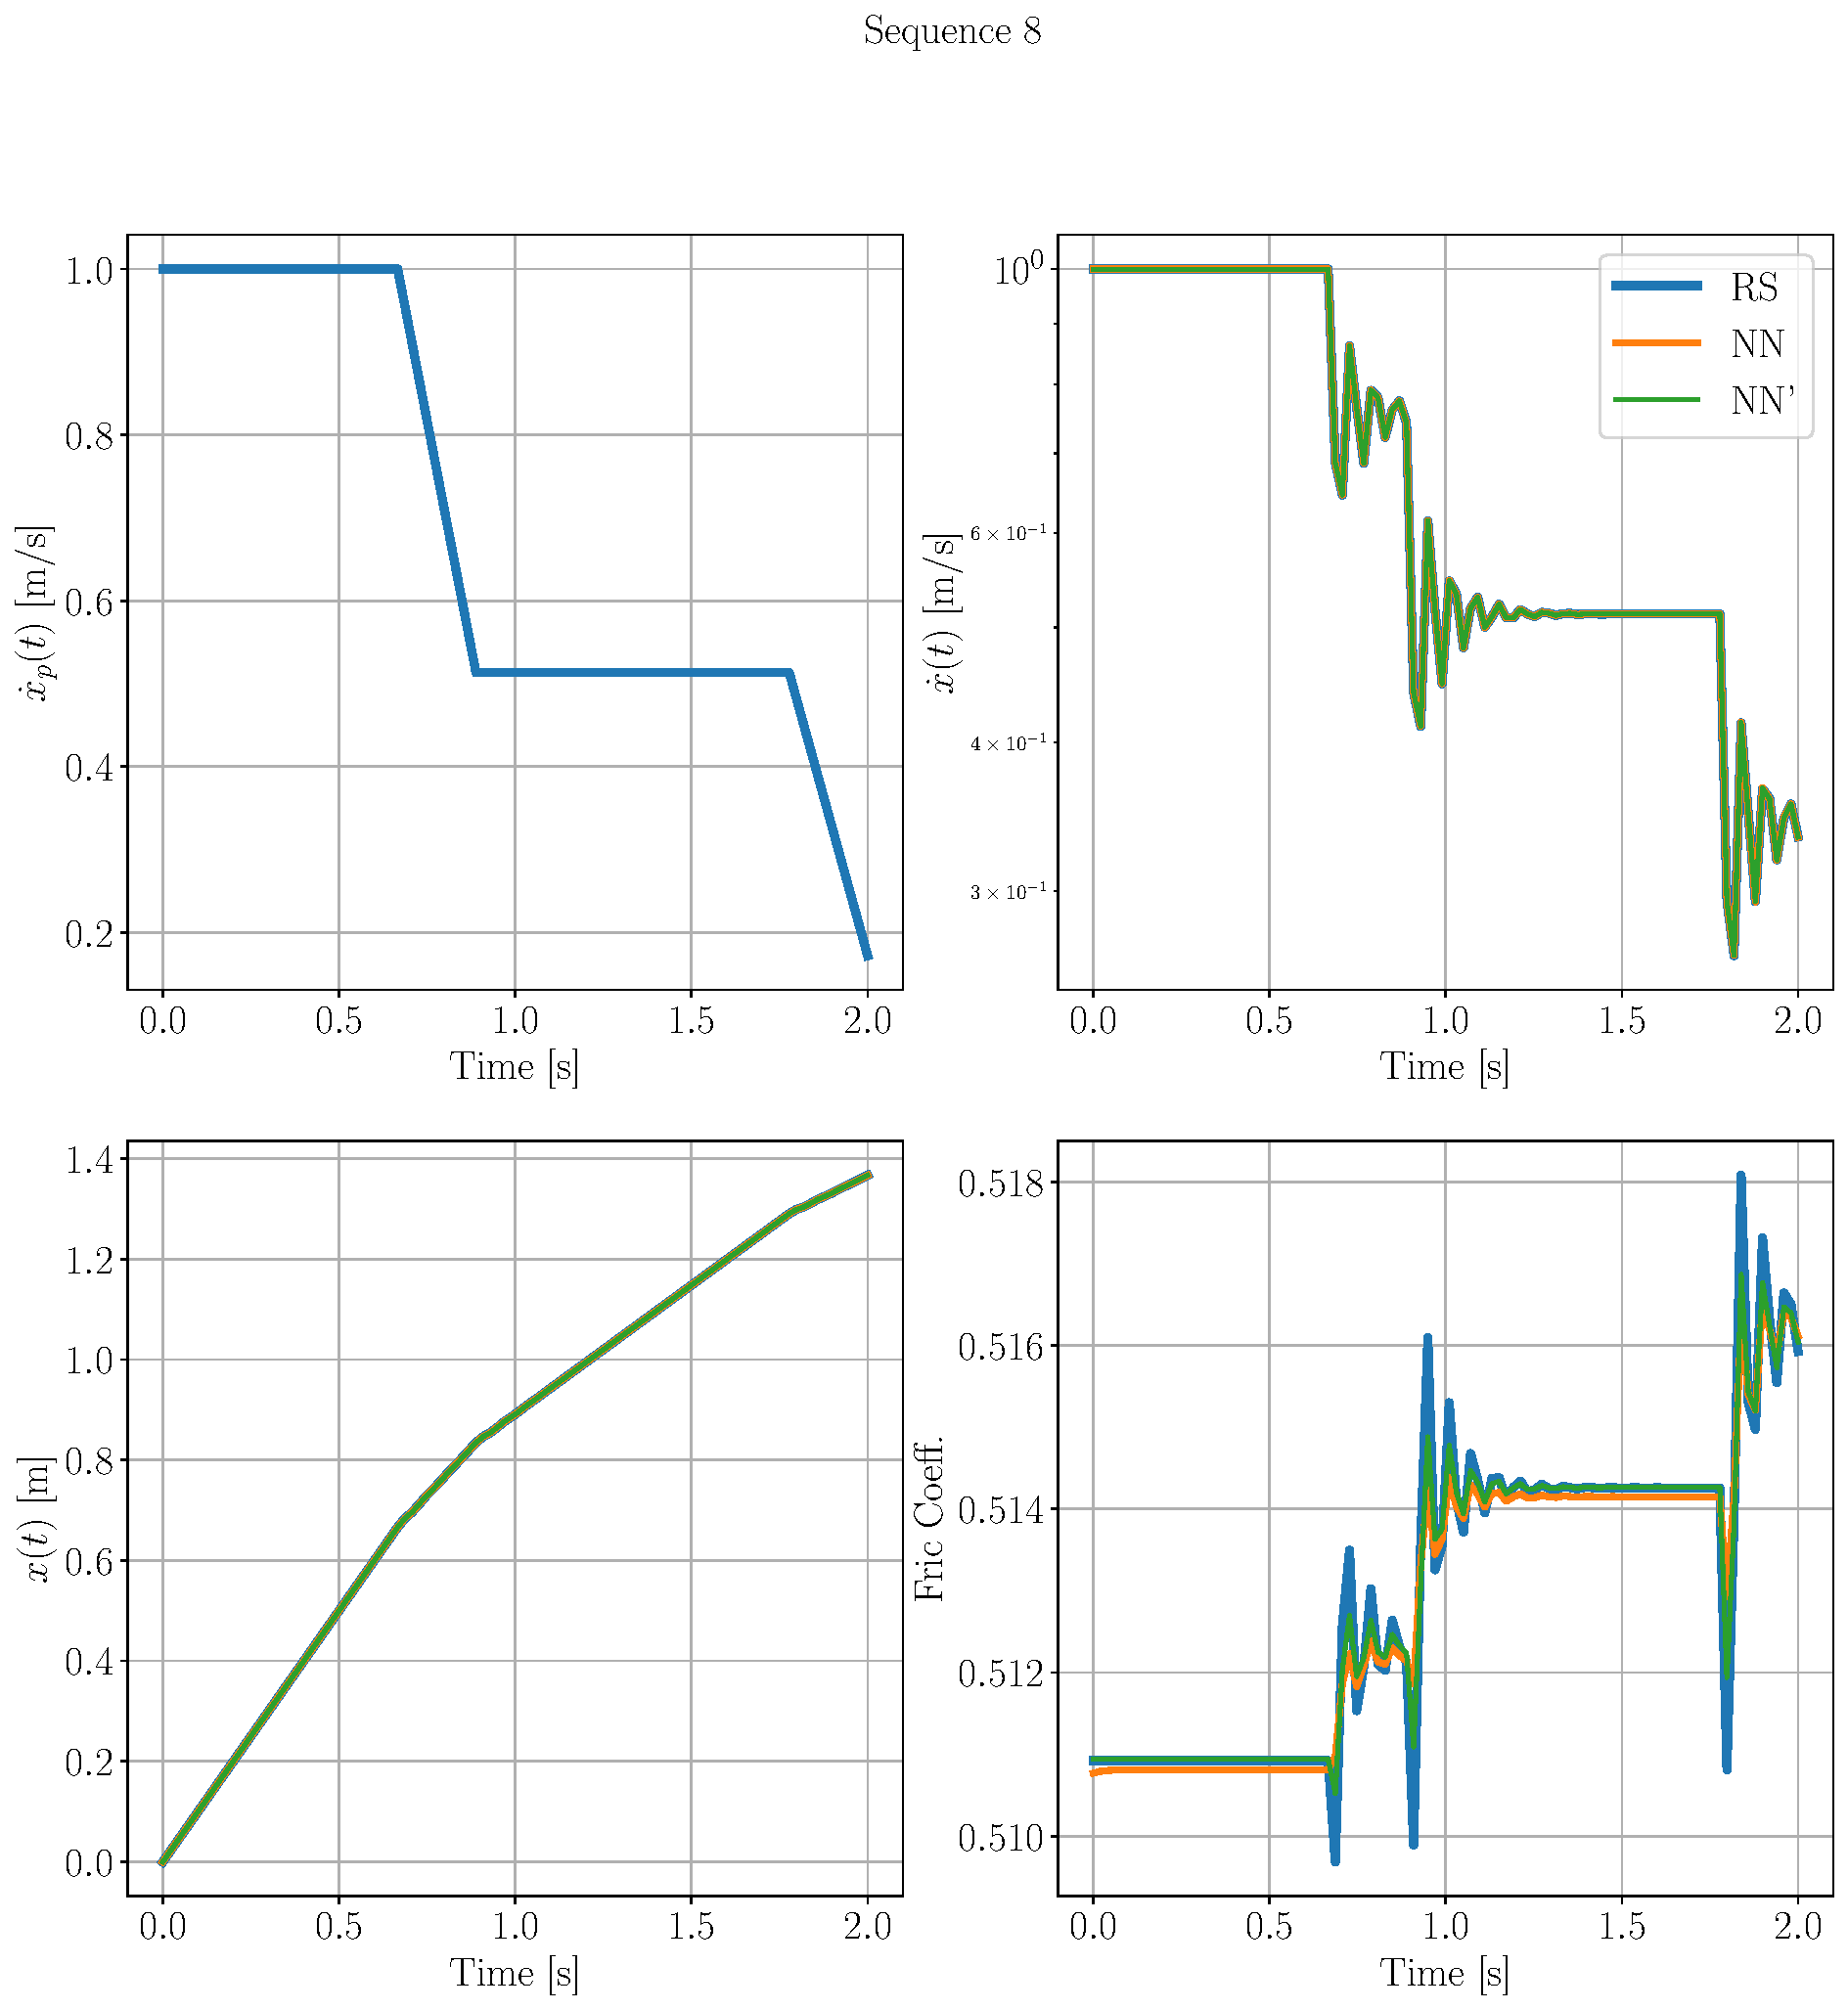
\includegraphics[width=0.9\textwidth]{figures/SS_seq8_0216_0521SS_combined_800.pdf}
    \caption{An example sequence of spring-slider solution with original rate-and-state friction, 
    NN potentials, 
    and NN potentials further trained on spring-slider sequences}
    \label{fig:SSseq8}
\end{figure}

\begin{table}[htbp]
    \centering
    \begin{tabular}{ccc}
        \hline
        Solution term & NN & NN' \\
        \hline
        $x(t)$ & $(1.9 \pm 1.8)\times 10^{-5}$ & $(5.4 \pm 4.4 )\times 10^{-6}$\\
        $\dot{x}(t)$ & $(2.7 \pm 3.6)\times 10^{-4}$ & $(1.6 \pm 2.2)\times 10^{-4}$\\
        $f(t)$ & $0.030 \pm 0.024$ & $0.016 \pm 0.016$\\
        \hline
    \end{tabular}
    \caption{Testing relative $L_2$ error for the original potentials only trained on velocity-jump and continuous variation dataset (NN), 
    updated potentials further trained on 200 spring-slider like dataset (NN'). 
    averaged over 10 test spring-slider sequences. }
    \label{tab:NNvsNNPrime}
\end{table}

The potential formulated friction is that it can solve all the sequences, 
with either explicit or implicit solver.  
In contrast the original rate-and-state friction fails to solve over $60\%$ of the sequences at even the finest $\Delta t$ with the implicit solver, 
and over $40\%$ with the explicit solver. 
Table~\ref{tab:NaNRatioSpringSliderRsVsNNRespective} lists the ratio of sequences that cannot be solved by each (NN/RS, ex/implicit) pair. 

\begin{table}[H]
    \centering
    \begin{tabular}{cccccccc}
        \hline
        $\Delta t$ [s] & $2^{-13.5}$ & $2^{-13.0}$ & $2^{-12.5}$ & $2^{-12.0}$ & $2^{-11.5}$ & $2^{-11.0}$ \\
        \hline
        NN, implicit & 0.000 & 0.000 & 0.000 & 0.000 & 0.000 & 0.000 \\
        NN, explicit & 0.000 & 0.000 & 0.000 & 0.000 & 0.000 & 0.000 \\
        RS, implicit & 0.506 & 0.571 & 0.623 & 0.623 & 0.675 & 0.727 \\
        RS, explicit & 0.455 & 0.455 & 0.455 & 0.455 & 0.455 & 0.455 \\
        \hline
    \end{tabular}
    \caption{Ratio of sequences that cannot be solved by NN, RS models with implicit, explicit solvers.}
    \label{tab:NaNRatioSpringSliderRsVsNNRespective}
\end{table}

The fact that rate-and-state friction does not converge with the implicit solver is non-surprising given that it does not have an associated energy formulation. 
The fact that the potential formulated friction works well with the implicit solver is consistent with (\ref{eq:JfunctionalMin}) being a convex minimization problem. 

Next, 
we check the growth of error as $\Delta t$ increases for those sequences that (NN, implicit), (NN, explicit) and (RS, explicit) can all solve. 
Since we do not have analytical solutions for the sequences, 
Error is computed against the solve with the finest $\delta t = 2^{-14}\ \mathrm{s}$, for each (model, ex/implicit) pair. 
Figure~\ref{fig:ErrGrowthDt} shows that the error in $\dot{x}(t)$ is on the order of $10^{-5}$, 
while further increasing $\Delta t$ would result in (RS, explicit) not solving some of the sequences listed here. 
We conclude that within this range of $\Delta t$ such that all the three pairs can solve these sequences, 
their error growth is comparable and small, 
since the fitting error between potential formulated friction and rate-and-state friction is already on the order of $10^{-4}$. 
For the sequences that (RS, explicit) cannot solve, 
further decreasing the time step to $\Delta t = 2^{-19}\approx 10^{-6}\ \mathrm{s}$ still will not solve them, 
while further decreasing $\Delta t$ is of little practical value since that is close to the precision of float tensors on GPUs. 

Detailed error can be found in Table~\ref{tab:MeanL2ErrorSpringSliderRsVsNNRespective} and \ref{tab:StdL2ErrorSpringSliderRsVsNNRespective}.
\begin{figure}
    \centering
    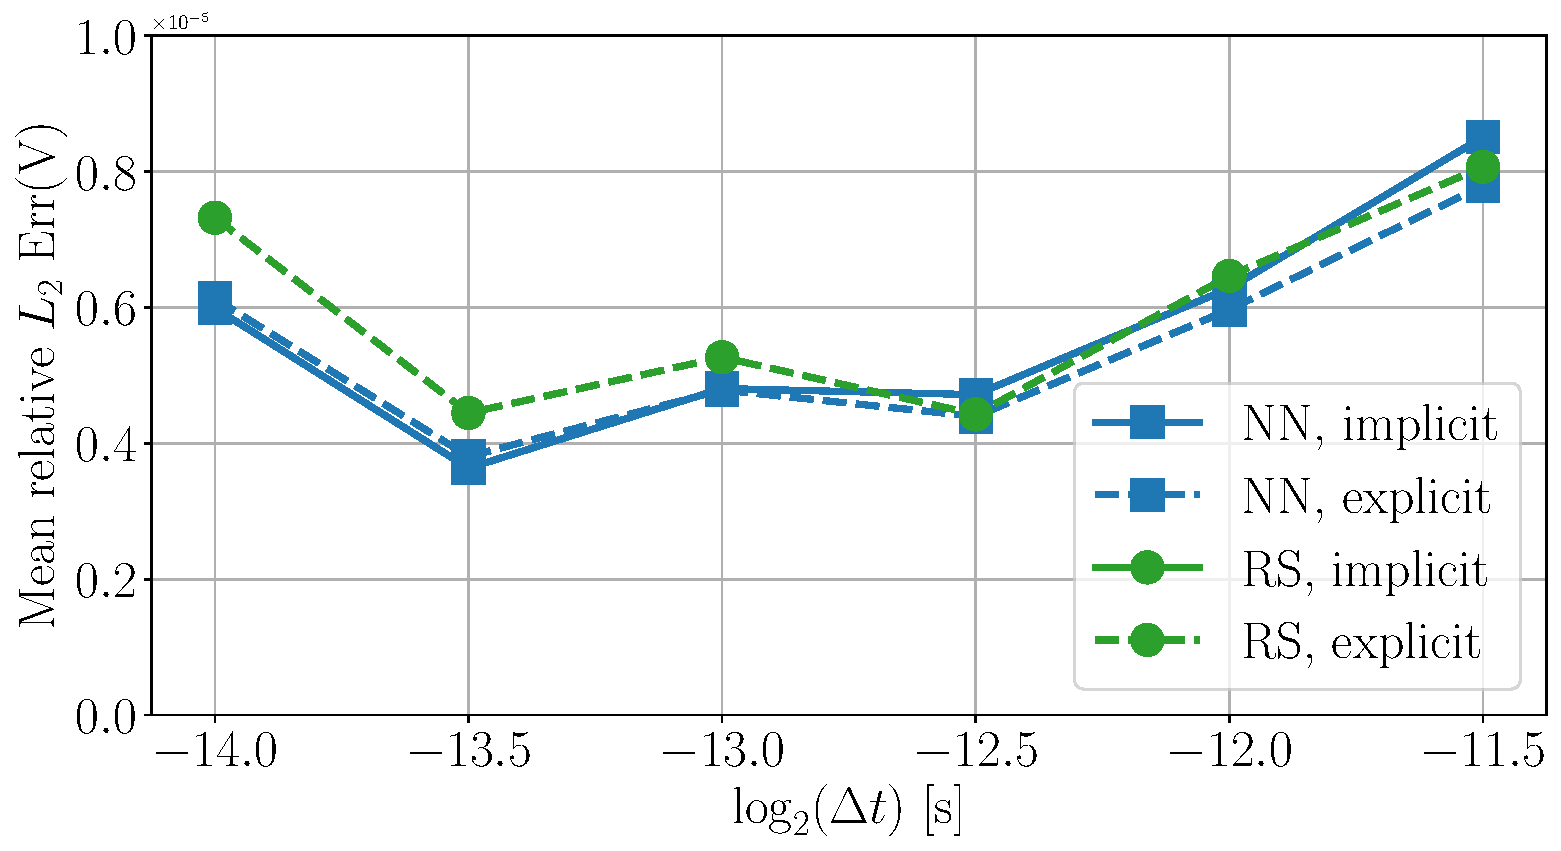
\includegraphics[width=0.7\textwidth]{figures/ErrGrowthDeltaT.pdf}
    \caption{Growth of relative $L_2$ error in $\dot{x}(t)$ as $\Delta t$ increases. 
    Note that since (RS, implicit) cannot solve some of the sequences that the other three pairs can solve, 
    its error is not plotted here.}
    \label{fig:ErrGrowthDt}
\end{figure}


\section{Conclusions}
\label{sec:conclusions}
\ifincludetext{
In this study, 
we have developed a potential-formulated friction that resembles the widely-used rate-and-state friction law. 
By constructing the potentials using Recurrent Neural Operators (RNOs) and training them on generated rate-and-state slip-friction sequences, 
we have verified that the potential friction formulation can capture the history dependencies well in rate-and-state friction, 
which is widely observed from experimental data. 
This suggests that there exists a potential-formulated friction law of our specific form that approximates the empirical rate-and-state friction well, 
with a relative $L_2$ error in friction coefficient of $2 \times 10^{-4}$. 
This is 2 orders of magnitude lower than the error between the best rate-and-state friction fit to real experimental data, 
which implies that they likely will fit the experimental data similarly well. 
We testify through different training runs that in our potential formulation, hidden variable $\xi$ is unique up to affine transformations.

We have also confirmed by solving spring-slider systems that the potential friction formulation can facilitate implicit solves of initial value problems with rate-and-state frictional interfaces, 
since the propagation of solution to the next time step can be written as a convex minimization problem. 
We test whether or not the proposed potential formulation facilitates implicit solves of initial value problems by solving spring-slider dynamic problems under displacement-control loading. 
We sample $77$ sequences with different spring constants and loading, 
and out of them rate-and-state friction cannot solve over $50\%$ of the sequences with implicit solver, $46\%$ of the sequences with explicit solver. 
While potential-formulated friction can solve all of these sequences, 
with either implicit or explicit solver. 
For the explicit solver, 
rate-and-state friction still cannot solve those sequences with a time step $1/256$ of that of the potential-formulated friction.  ($2^{-19}$ vs $2^{-11}\ \mathrm{s}$). 
Within the sequences that both explicit rate-and-state and implicit potential friction can solve, 
they achieve similar accuracy as time step increases. 

With all the advantages of the potential formulation for rate-and-state friction, 
there is one drawback worth mentioning. 
The potentials require a large number of sequences in the training dataset to achieve good test error. 
Since compared to the original rate-and-state friction law, 
there are much more parameters in the potentials from their Neural Network structure, 
hundreds of sequences are required to avoid over-fitting and achieve good test error. 
In practice, 
it is sometimes difficult to obtain hundreds of sequences from experiments done on the same frictional interface, 
while the original rate-and-state friction law in general requires a handful of sequences to fit the four parameters. 

In the future, 
we would work on finding closed-form approximations to the learnt potentials, 
such that taking their gradients can be done more time-efficiently. 
Right now since the potentials are still neural networks, 
the differentiation process is time consuming. 
We would work on fitting the potential formulations directly to experimental measurements and compare the fitting error with the original rate-and-state formulation. 
}
\fi
%% The Appendices part is started with the command \appendix;
%% appendix sections are then done as normal sections
\newpage
\appendix
\section{Supplementary figures and tables}
\begin{figure}[htb!]
    \centering
    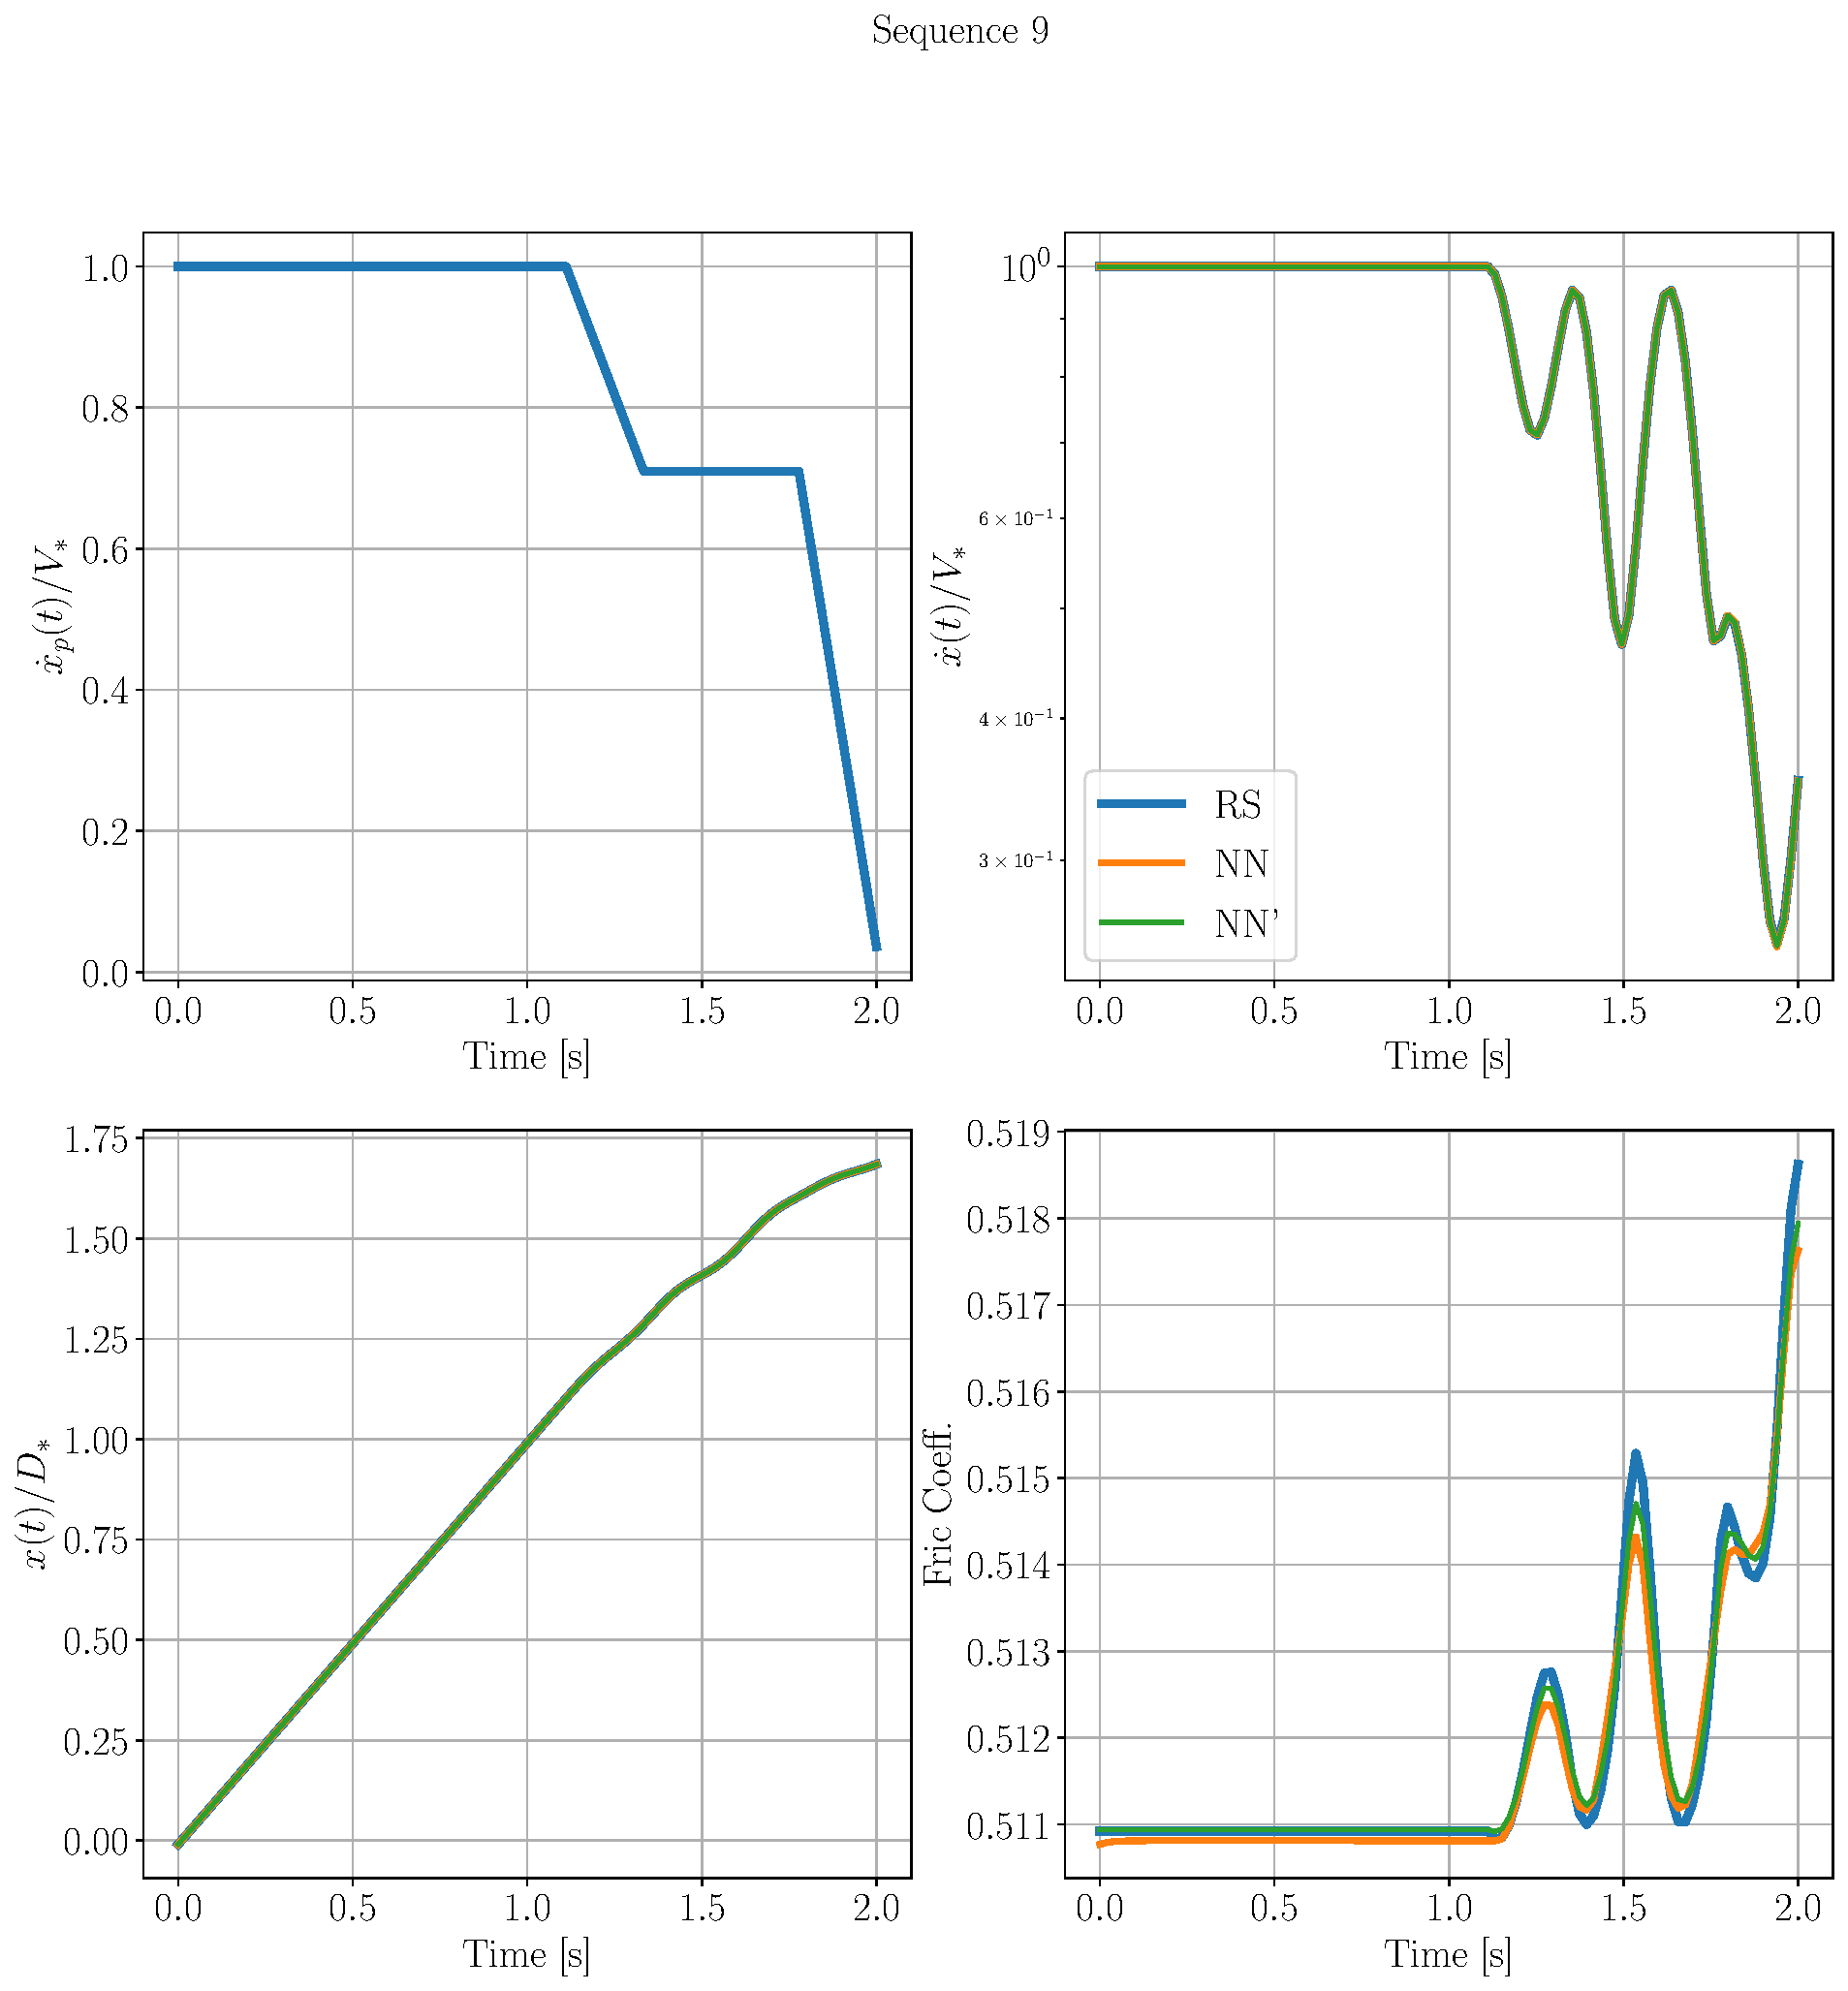
\includegraphics[width=0.9\textwidth]{SS_seq9_0216_0521SS_combined_800.pdf}
    \caption{An example sequence of spring-slider solution with original rate-and-state friction, 
    NN potentials, 
    and NN potentials further trained on spring-slider sequences}
    \label{fig:SSseq9}
\end{figure}

\begin{table}[htb!]
    \centering
    \begin{tabular}{ccccccc}
        \hline
        $\Delta t$ [s] & $2^{-13.5}$ & $2^{-13.0}$ & $2^{-12.5}$ & $2^{-12.0}$ & $2^{-11.5}$ & $2^{-11.0}$ \\
        \hline
        NN, implicit & 5.993e-06 & 3.636e-06 & 4.807e-06 & 4.716e-06 & 6.282e-06 & 8.508e-06 \\
        NN, explicit & 6.130e-06 & 3.808e-06 & 4.786e-06 & 4.397e-06 & 5.968e-06 & 7.795e-06 \\
        RS, implicit & nan & nan & nan & nan & nan & nan \\
        RS, explicit & 7.321e-06 & 4.447e-06 & 5.267e-06 & 4.426e-06 & 6.464e-06 & 8.069e-06 \\
        \hline
    \end{tabular}
    \caption{Mean relative $L_2$ error in $\dot{x}(t)$ averaged over 77 sequences, 
    for NN, RS models with implicit, explicit solvers.}
    \label{tab:MeanL2ErrorSpringSliderRsVsNNRespective}
\end{table}

\begin{table}[htb!]
    \centering
    \begin{tabular}{cccccccc}
        \hline
        $\Delta t$ [s] & $2^{-13.5}$ & $2^{-13.0}$ & $2^{-12.5}$ & $2^{-12.0}$ & $2^{-11.5}$ & $2^{-11.0}$ \\
        \hline
        NN, implicit & 5.799e-06 & 5.390e-06 & 5.575e-06 & 7.069e-06 & 6.384e-06 & 1.033e-05 \\
        NN, explicit & 6.241e-06 & 5.766e-06 & 5.844e-06 & 6.887e-06 & 6.572e-06 & 9.639e-06 \\
        RS, implicit & nan & nan & nan & nan & nan & nan \\
        RS, explicit & 9.601e-06 & 6.886e-06 & 5.541e-06 & 5.597e-06 & 6.845e-06 & 1.017e-05 \\
        \hline
    \end{tabular}
    \caption{Standard deviation of relative $L_2$ error in $\dot{x}(t)$ over 77 sequences, 
    for NN, RS models with implicit, explicit solvers.}
    \label{tab:StdL2ErrorSpringSliderRsVsNNRespective}
\end{table}


%% If you have bibdatabase file and want bibtex to generate the
%% bibitems, please use
%%
\newpage
 \bibliographystyle{elsarticle-num} 
 \bibliography{cas-refs}

\end{document}
